% Options for packages loaded elsewhere
\PassOptionsToPackage{unicode}{hyperref}
\PassOptionsToPackage{hyphens}{url}
\documentclass[
  ignorenonframetext,
]{beamer}
\newif\ifbibliography
\usepackage{pgfpages}
\setbeamertemplate{caption}[numbered]
\setbeamertemplate{caption label separator}{: }
\setbeamercolor{caption name}{fg=normal text.fg}
\beamertemplatenavigationsymbolsempty
% remove section numbering
\setbeamertemplate{part page}{
  \centering
  \begin{beamercolorbox}[sep=16pt,center]{part title}
    \usebeamerfont{part title}\insertpart\par
  \end{beamercolorbox}
}
\setbeamertemplate{section page}{
  \centering
  \begin{beamercolorbox}[sep=12pt,center]{section title}
    \usebeamerfont{section title}\insertsection\par
  \end{beamercolorbox}
}
\setbeamertemplate{subsection page}{
  \centering
  \begin{beamercolorbox}[sep=8pt,center]{subsection title}
    \usebeamerfont{subsection title}\insertsubsection\par
  \end{beamercolorbox}
}
% Prevent slide breaks in the middle of a paragraph
\widowpenalties 1 10000
\raggedbottom
\AtBeginPart{
  \frame{\partpage}
}
\AtBeginSection{
  \ifbibliography
  \else
    \frame{\sectionpage}
  \fi
}
\AtBeginSubsection{
  \frame{\subsectionpage}
}
\usepackage{iftex}
\ifPDFTeX
  \usepackage[T1]{fontenc}
  \usepackage[utf8]{inputenc}
  \usepackage{textcomp} % provide euro and other symbols
\else % if luatex or xetex
  \usepackage{unicode-math} % this also loads fontspec
  \defaultfontfeatures{Scale=MatchLowercase}
  \defaultfontfeatures[\rmfamily]{Ligatures=TeX,Scale=1}
\fi
\usepackage{lmodern}
\ifPDFTeX\else
  % xetex/luatex font selection
\fi
% Use upquote if available, for straight quotes in verbatim environments
\IfFileExists{upquote.sty}{\usepackage{upquote}}{}
\IfFileExists{microtype.sty}{% use microtype if available
  \usepackage[]{microtype}
  \UseMicrotypeSet[protrusion]{basicmath} % disable protrusion for tt fonts
}{}
\makeatletter
\@ifundefined{KOMAClassName}{% if non-KOMA class
  \IfFileExists{parskip.sty}{%
    \usepackage{parskip}
  }{% else
    \setlength{\parindent}{0pt}
    \setlength{\parskip}{6pt plus 2pt minus 1pt}}
}{% if KOMA class
  \KOMAoptions{parskip=half}}
\makeatother
\usepackage{graphicx}
\makeatletter
\newsavebox\pandoc@box
\newcommand*\pandocbounded[1]{% scales image to fit in text height/width
  \sbox\pandoc@box{#1}%
  \Gscale@div\@tempa{\textheight}{\dimexpr\ht\pandoc@box+\dp\pandoc@box\relax}%
  \Gscale@div\@tempb{\linewidth}{\wd\pandoc@box}%
  \ifdim\@tempb\p@<\@tempa\p@\let\@tempa\@tempb\fi% select the smaller of both
  \ifdim\@tempa\p@<\p@\scalebox{\@tempa}{\usebox\pandoc@box}%
  \else\usebox{\pandoc@box}%
  \fi%
}
% Set default figure placement to htbp
\def\fps@figure{htbp}
\makeatother
\setlength{\emergencystretch}{3em} % prevent overfull lines
\providecommand{\tightlist}{%
  \setlength{\itemsep}{0pt}\setlength{\parskip}{0pt}}
% Slide layout defaults for warning-clean scientific decks.
\usepackage{etoolbox}
\IfFileExists{xurl.sty}{\usepackage{xurl}}{}
\IfFileExists{seqsplit.sty}{\usepackage{seqsplit}}{\newcommand{\seqsplit}[1]{#1}}
\protected\def\breakseq#1{\seqsplit{#1}}
\protected\def\breaktt#1{\begingroup\ttfamily\seqsplit{#1}\endgroup}
\setlength{\emergencystretch}{6em}
\tolerance=5000
\hbadness=10000
\hfuzz=1pt
\setlength{\tabcolsep}{2pt}
\AtBeginEnvironment{longtable}{\tiny\renewcommand{\arraystretch}{0.86}\setlength{\tabcolsep}{1pt}}
\AtBeginEnvironment{tabular}{\tiny\renewcommand{\arraystretch}{0.86}\setlength{\tabcolsep}{1pt}}

% Natbib and cross-reference fallbacks — slides don't load natbib
% or cleveref, but combined-PDF manuscript prose may emit these
% commands. The fallback renders citations as a bracketed key list
% and cross-references as detokenized labels so slides don't fail on
% undefined control sequences or raw underscores. \providecommand is
% a no-op if packages load later.
\providecommand{\citep}[1]{[#1]}
\providecommand{\citet}[1]{#1}
\providecommand{\citealp}[1]{#1}
\providecommand{\citeauthor}[1]{#1}
\providecommand{\citeyear}[1]{#1}
\providecommand{\cref}[1]{\texttt{\detokenize{#1}}}
\providecommand{\Cref}[1]{\texttt{\detokenize{#1}}}

\newtheorem{proposition}{Proposition}
\newtheorem{hypothesis}{Hypothesis}
\usepackage{bookmark}
\IfFileExists{xurl.sty}{\usepackage{xurl}}{} % add URL line breaks if available
\urlstyle{same}
% fallback for those not using the hyperref driver hyperxmp:
\makeatletter
\@ifundefined{xmpquote}{\newcommand{\xmpquote}[1]{#1}}{}
\makeatother
\hypersetup{
  hidelinks,
  pdfcreator={LaTeX via pandoc}}

\author{\texorpdfstring{}{}}
\date{}

\begin{document}

\section{Methods Protocol: Governance, Provenance, and
Validation}\label{sec:methods_protocol}

\begin{frame}[fragile,allowframebreaks]{Event Logging and
Participant-Facing Governance}
\protect\phantomsection\label{event-logging-and-participant-facing-governance}
DigiPPPiP is presented as a framework manuscript, so its method layer is
a protocol specification rather than a participant dataset. The protocol
requires timestamped events with actor, action, and channel fields; the
example trace in \breakseq{[@fig:event\_logging\_schema]} has 6 summary fields,
a mean interval of 4 seconds, and a turn-balance score of 1. This makes
the distinction among synchronous, semisynchronous, and asynchronous
sessions auditable instead of rhetorical. The same event stream supports
replay, accessibility auditing, outcome modeling, and synchronization
with optional physiological channels, but those uses must stay visibly
downstream from the partner-facing mark.

Digital pen and paper research in observational settings gives a
practical precedent for treating pen traces as analyzable field records
rather than merely as drawings \breakseq{[@weibel2012digitalpen]}. DigiPPPiP
extends that idea to a dyadic protocol: the stroke is simultaneously a
mark for the partner, an event for replay, and a data row for later
audit. That dual role is why the manuscript separates the visible canvas
from the event log, source ledger, and generated figure registry.

\breakseq{[@fig:event\_logging\_schema]} now treats the method layer as an
end-to-end data-flow contract. Raw partner actions are captured as
consented event rows, separated from the visible canvas and replay
record, transformed into summaries, optionally modeled, rendered as
figures and variables, governed by claim/source/readiness audits, and
finally published through the template pipeline. The important
architectural rule is separation: human-authored marks, optional AI
outputs, computed diagnostics, and publication artifacts should remain
distinguishable in both the protocol and the figures.

\begin{figure}
\centering
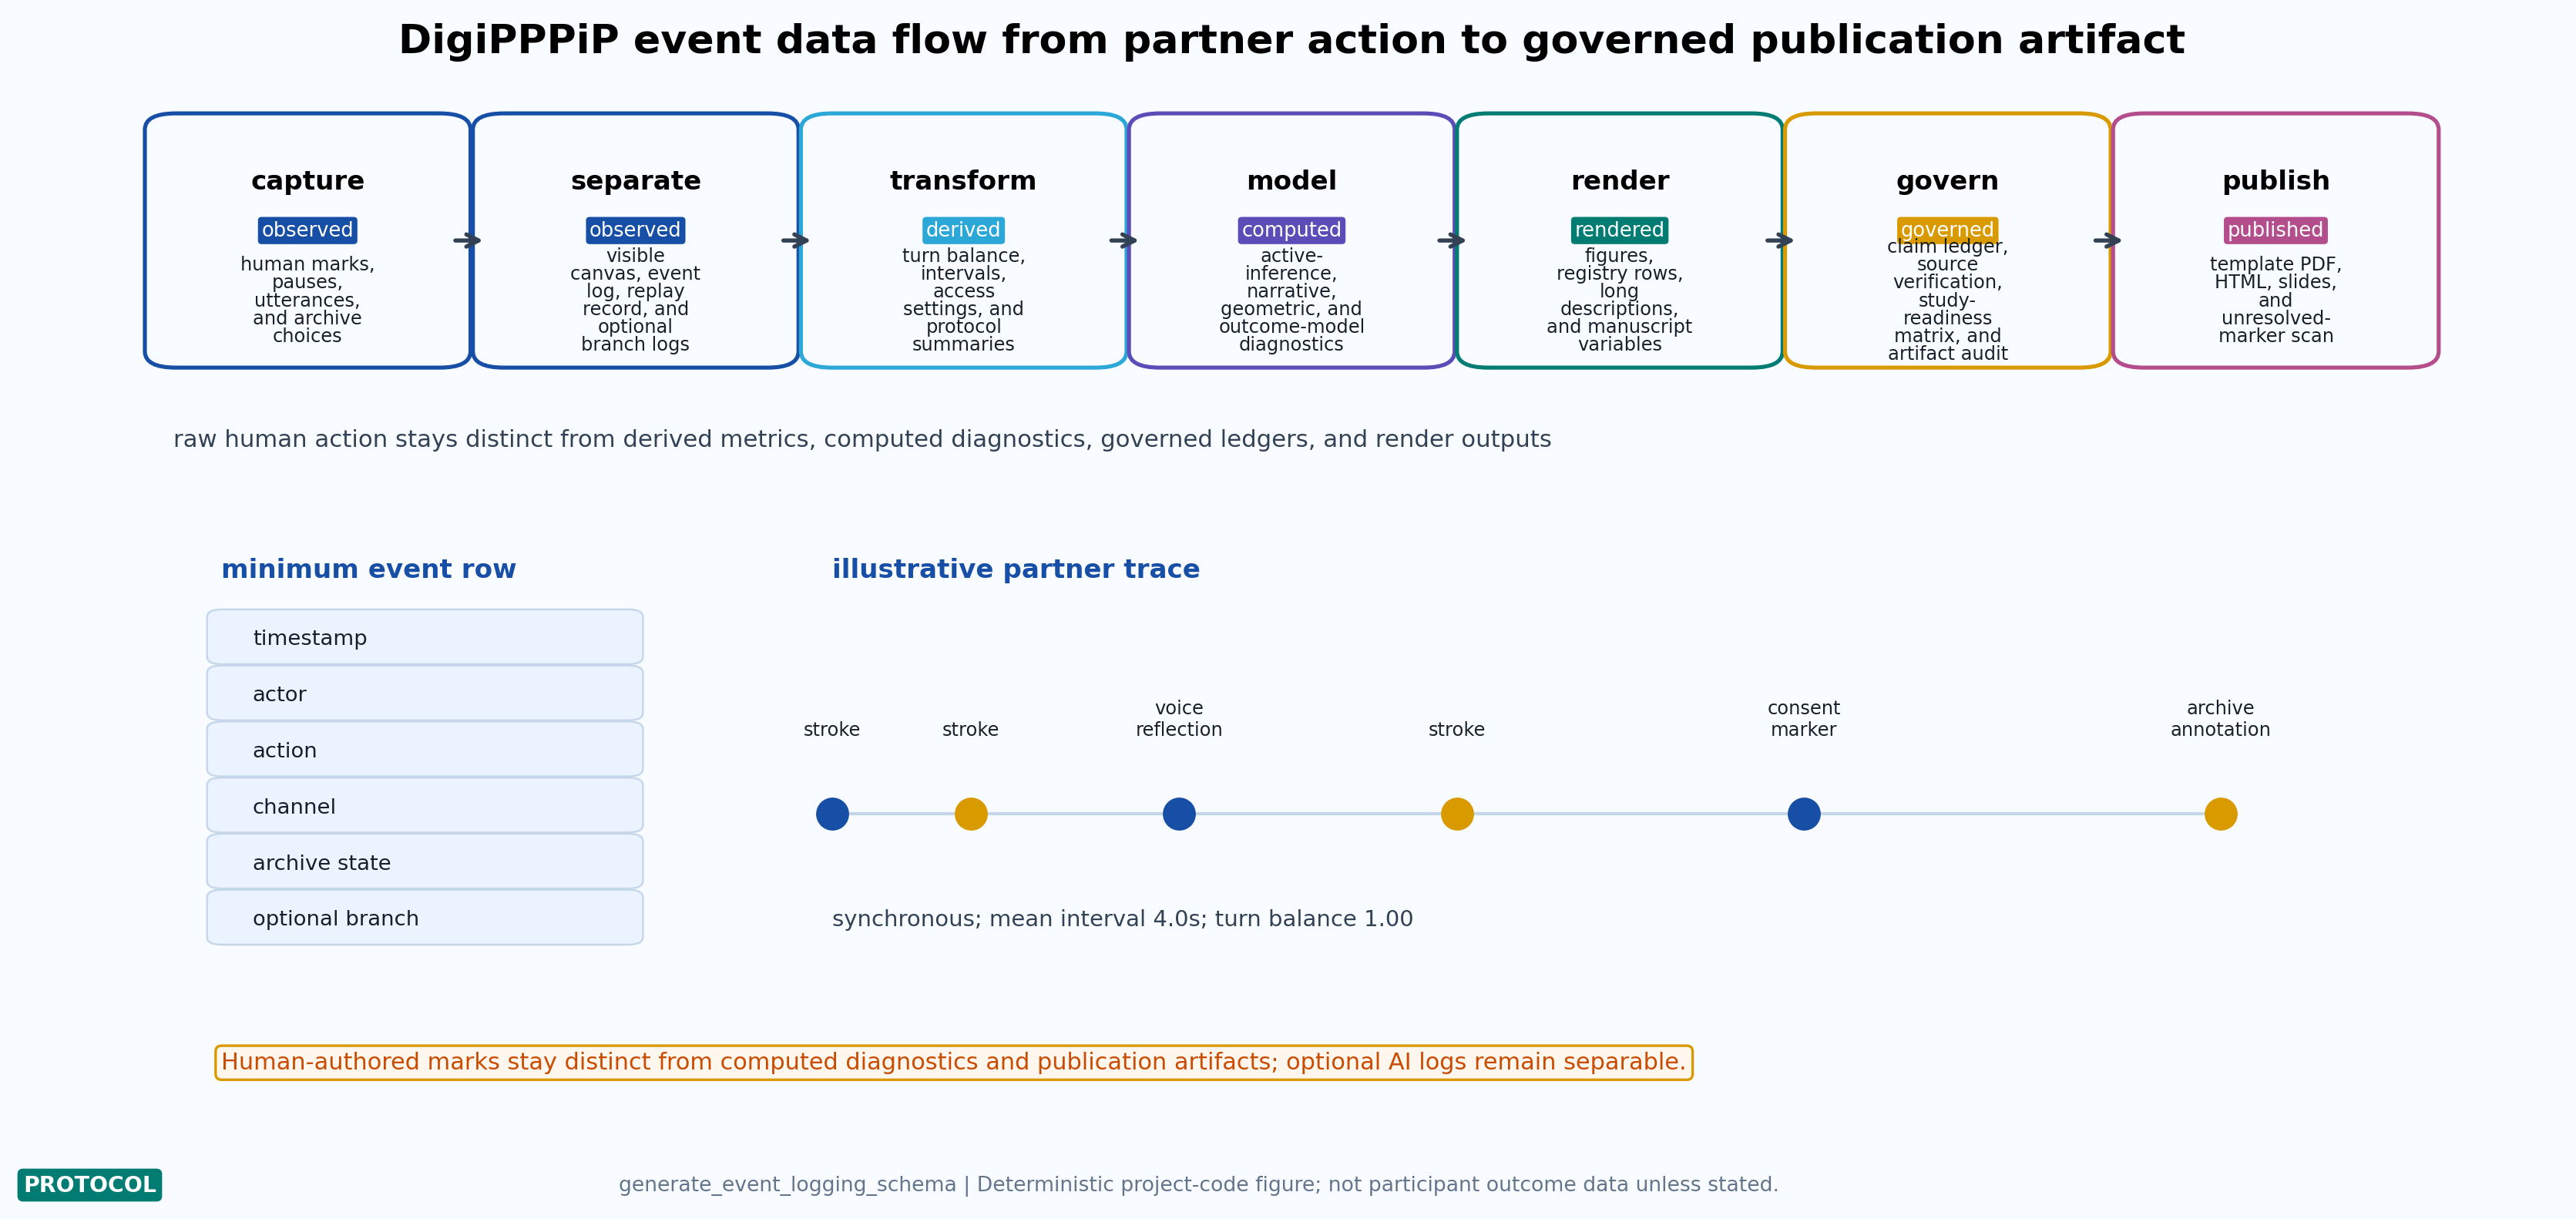
\includegraphics[width=0.95\linewidth,height=0.46\textheight,keepaspectratio,alt={Event schema, data-flow path, and example DigiPPPiP session trace. The figure is generated by generate\_event\_logging\_schema() from src/session\_events.py and src/systems\_governance.py; read the top row as the capture-to-publication path, the lower-left list as minimum event-row fields, and the timeline as an illustrative actor/action sequence with temporal summary metrics. It supports the protocol claim that synchrony categories, model diagnostics, generated figures, and publication artifacts must remain auditable. The trace is illustrative, and participant studies would replace it with consented logs while keeping optional AI and physiology logs separable.}]{../figures/event_logging_schema.png}
\caption{Event schema, data-flow path, and example DigiPPPiP session
trace. The figure is generated by
\protect\breaktt{generate\_event\_logging\_schema()} from
\protect\breaktt{src/session\_events.py} and
\protect\breaktt{src/systems\_governance.py}; read the top row as the
capture-to-publication path, the lower-left list as minimum event-row
fields, and the timeline as an illustrative actor/action sequence with
temporal summary metrics. It supports the protocol claim that synchrony
categories, model diagnostics, generated figures, and publication
artifacts must remain auditable. The trace is illustrative, and
participant studies would replace it with consented logs while keeping
optional AI and physiology logs
separable.}\label{fig:event_logging_schema}
\end{figure}

Before human-subjects work, the protocol needs a participant-facing
layer as well as an analysis layer. The Common Rule and the Declaration
of Helsinki require consent, review, privacy, protocol clarity,
withdrawal, and risk handling to be explicit rather than inferred from
good intentions \breakseq{[@hhs2025cfr46; @wma2024helsinki]}. Digital-health
consent scholarship adds that participant understanding depends on
concrete information about access, purpose, privacy protection, and
oversight \breakseq{[@kassam2023digitalconsent]}. The plain-language brief
should say that two partners are invited to draw on a shared surface;
that the study records timing, tool, archive-control, and optional
replay events; that the activity is not treatment or a relationship
test; and that participants can pause, stop, withdraw, ask questions,
report discomfort, request redaction, and ask about save, replay,
export, and delete options before analysis lock. If one partner wants
more sharing and the other wants less, the stricter privacy choice
governs. This participant-facing appendix is generated as a protocol
artifact by \breaktt{src/study\_readiness.py} rather than left as
informal prose.

\breakseq{[@fig:study\_readiness\_matrix]} converts that ethics prose into a
protocol matrix. The rows are not optional decorations: they make dyadic
consent, deletion, export, replay, redaction, withdrawal, adverse-event
reporting, retention, disagreement handling, intervention description,
and optional AI-branch governance visible before recruitment.
Consent-forward digital mental-health work supports this placement
because archive controls need to be designed as user-facing choices
rather than hidden back-office data policy
\breakseq{[@pendse2024consentforward]}.

\begin{figure}
\centering
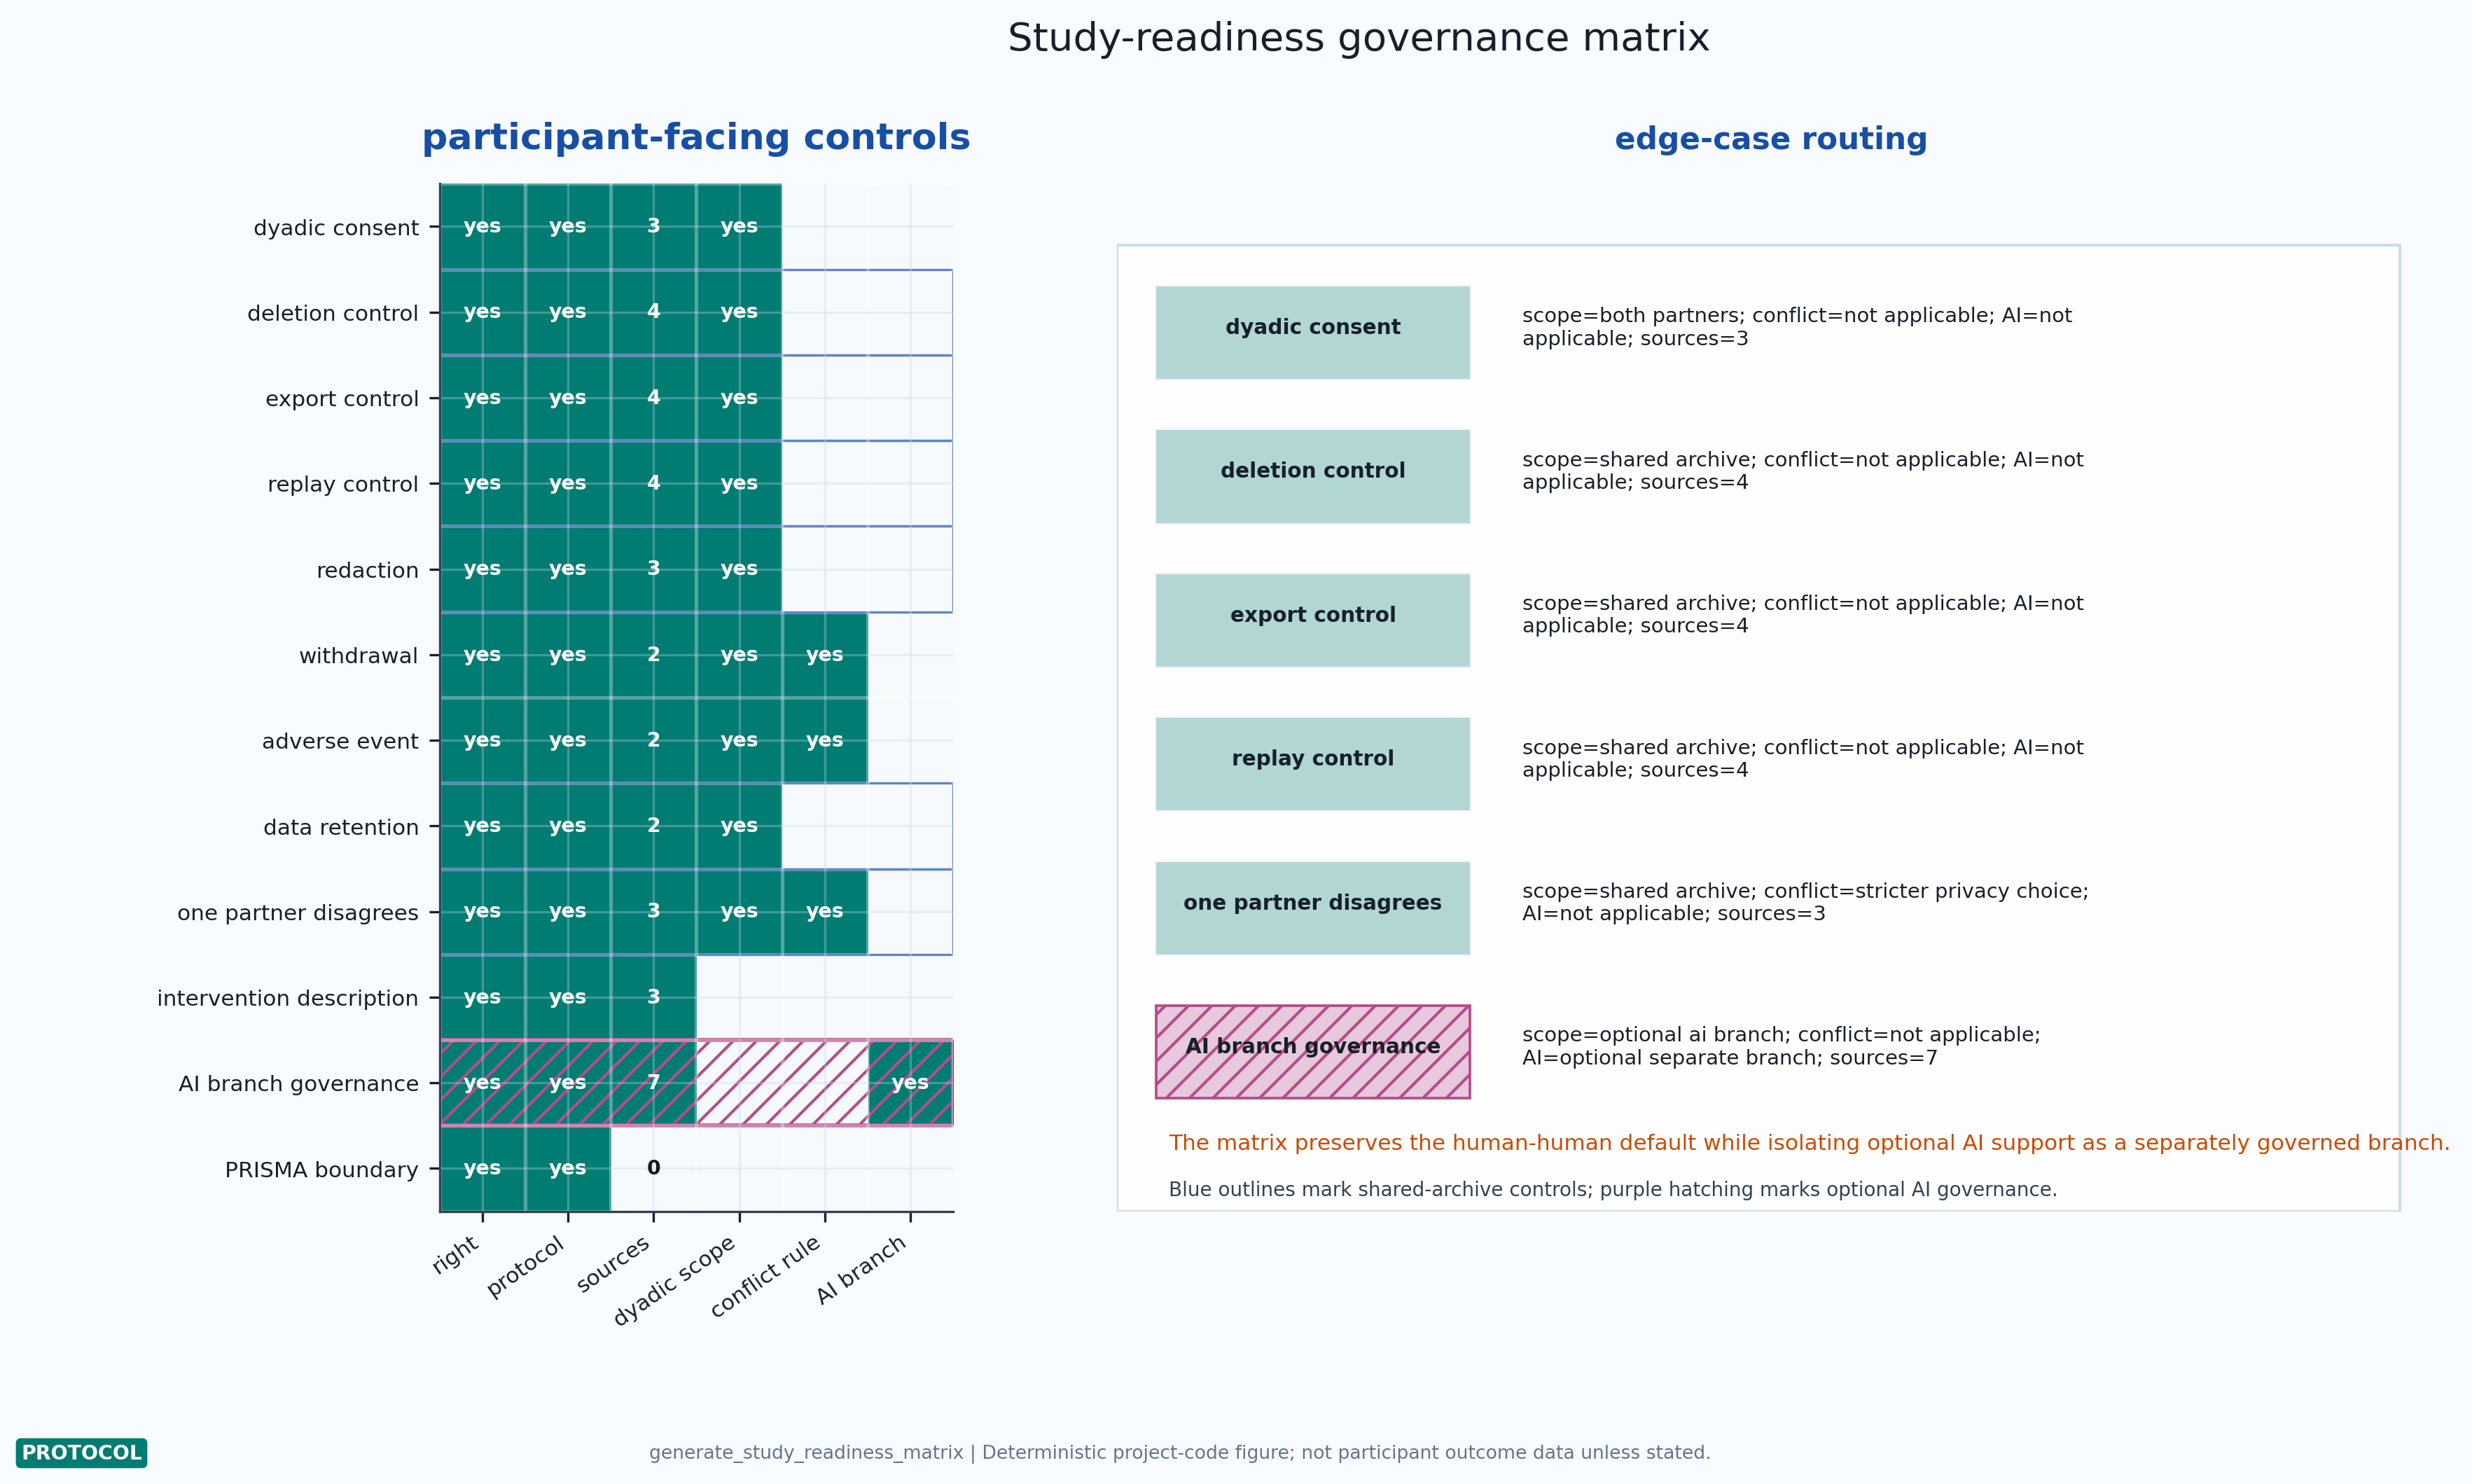
\includegraphics[width=0.95\linewidth,height=0.46\textheight,keepaspectratio,alt={Study-readiness governance matrix for DigiPPPiP. The figure is generated by generate\_study\_readiness\_matrix() from src/study\_readiness.py; read rows as protocol edge cases, green cells as text-labelled readiness commitments, source counts as anchor depth, blue outlines as shared-archive controls, purple hatching as optional AI governance, and the right panel as routing for deletion, export, replay, disagreement, and optional AI separation. It supports participant-facing readiness rather than study results. Empty cells mark controls that are not applicable to a given row, not missing duties.}]{../figures/study_readiness_matrix.png}
\caption{Study-readiness governance matrix for DigiPPPiP. The figure is
generated by \protect\breaktt{generate\_study\_readiness\_matrix()} from
\protect\breaktt{src/study\_readiness.py}; read rows as protocol edge
cases, green cells as text-labelled readiness commitments, source counts
as anchor depth, blue outlines as shared-archive controls, purple
hatching as optional AI governance, and the right panel as routing for
deletion, export, replay, disagreement, and optional AI separation. It
supports participant-facing readiness rather than study results. Empty
cells mark controls that are not applicable to a given row, not missing
duties.}\label{fig:study_readiness_matrix}
\end{figure}
\end{frame}

\begin{frame}[fragile,allowframebreaks]{Source and Claim Governance}
\protect\phantomsection\label{source-and-claim-governance}
The study protocol separates source quality from claim strength.
Peer-reviewed empirical and review articles can support scoped design
and measurement claims; books support theoretical framing; preprints and
reports are treated as provisional. \breakseq{[@fig:source\_quality\_map]}
encodes those rules so speculative additions, including geometric
hyperscanning and narrative-information proposals, are not used as
settled evidence. This is why digital object identifier (DOI)
verification matters: a search-result citation is not added unless
title, authors, venue, and DOI or stable uniform resource locator (URL)
match the intended claim. The stricter rule is claim-domain specific:
therapy, neural synchrony, active inference, accessibility, placemaking,
digital intimacy, AI mediation, and privacy persistence each have a
different maximum defensible claim strength before new evidence is
collected.

\begin{figure}
\centering
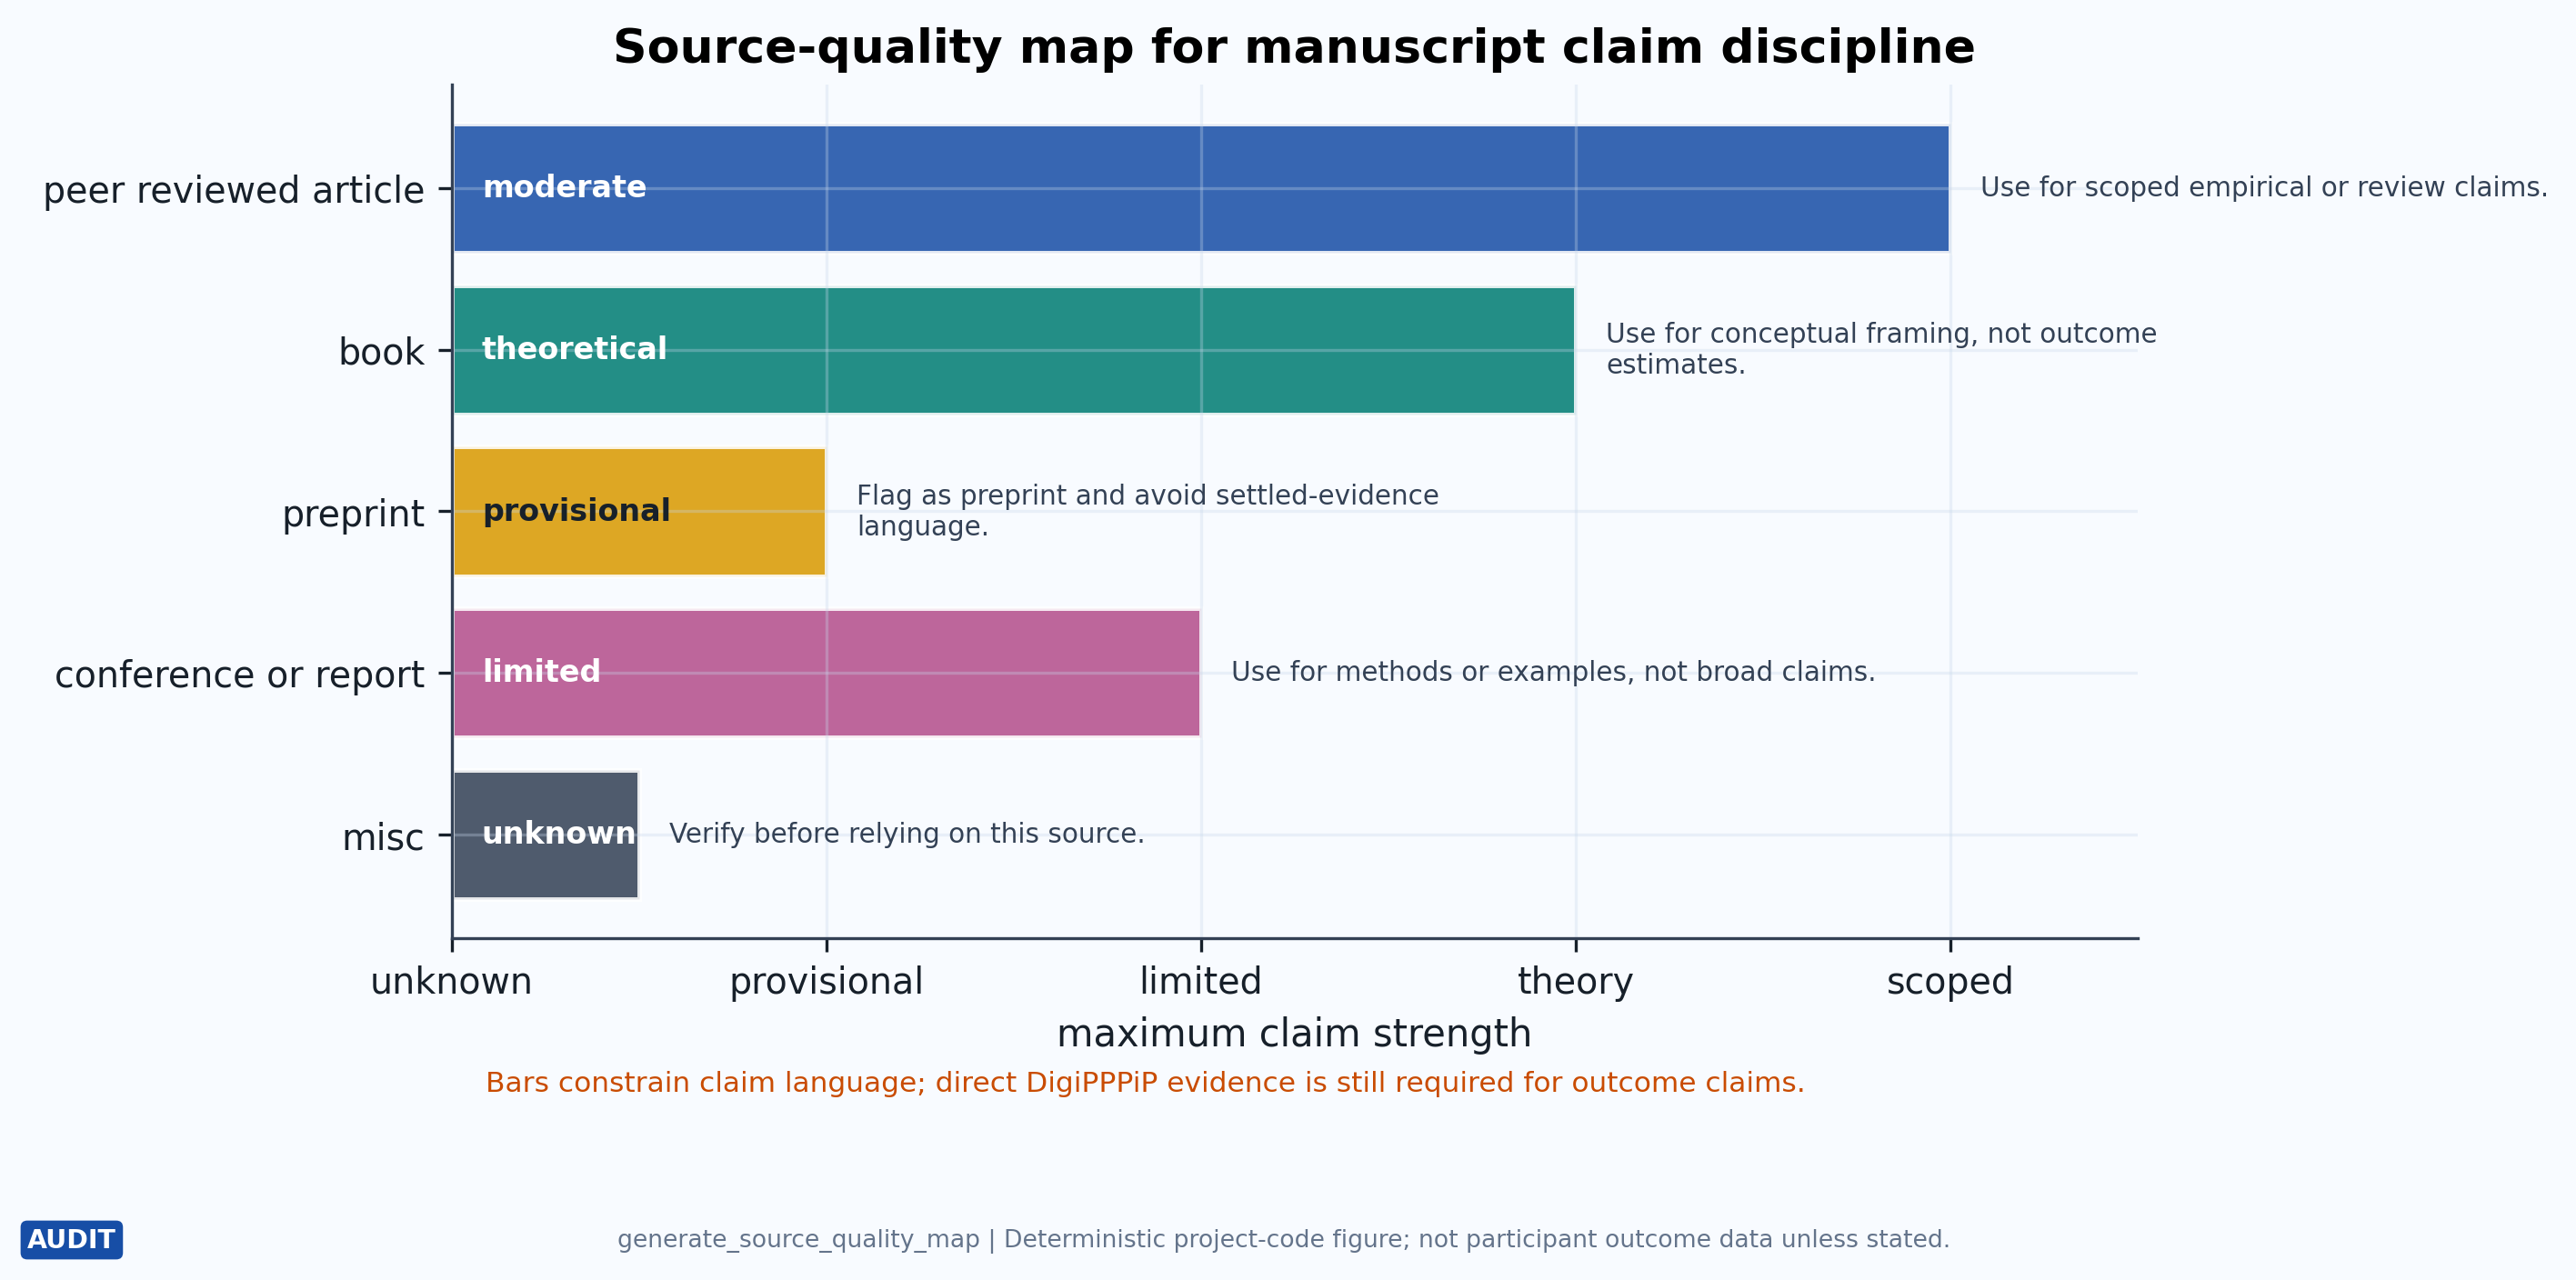
\includegraphics[width=0.9\linewidth,height=0.46\textheight,keepaspectratio,alt={Source-quality map for DigiPPPiP claim discipline. The figure is generated by generate\_source\_quality\_map() from src/source\_quality.py; read the horizontal bars as conservative maximum claim strength by source class, the embedded labels as source-tier roles, and the right-hand text as warnings for manuscript use. It supports the protocol rule that bibliography type constrains prose strength. The map is an audit device, not a judgment of individual papers, and claims can strengthen only with domain-appropriate empirical evidence.}]{../figures/source_quality_map.png}
\caption{Source-quality map for DigiPPPiP claim discipline. The figure
is generated by \protect\breaktt{generate\_source\_quality\_map()} from
\protect\breaktt{src/source\_quality.py}; read the horizontal bars as
conservative maximum claim strength by source class, the embedded labels
as source-tier roles, and the right-hand text as warnings for manuscript
use. It supports the protocol rule that bibliography type constrains
prose strength. The map is an audit device, not a judgment of individual
papers, and claims can strengthen only with domain-appropriate empirical
evidence.}\label{fig:source_quality_map}
\end{figure}

\breakseq{[@fig:claim\_boundary\_matrix]} makes that red-team layer explicit
across 14 recurring claim domains. The point is not to prohibit
ambitious studies; it is to keep the manuscript from borrowing strength
across domains. A valid shared-workspace source can motivate the
interface, but it cannot establish relationship improvement. A
hyperscanning method source can motivate instrumentation, but it cannot
establish causality or therapeutic benefit. A digital-art-therapy review
can motivate caution and study design, but it cannot turn DigiPPPiP into
treatment without direct evidence.

\begin{figure}
\centering
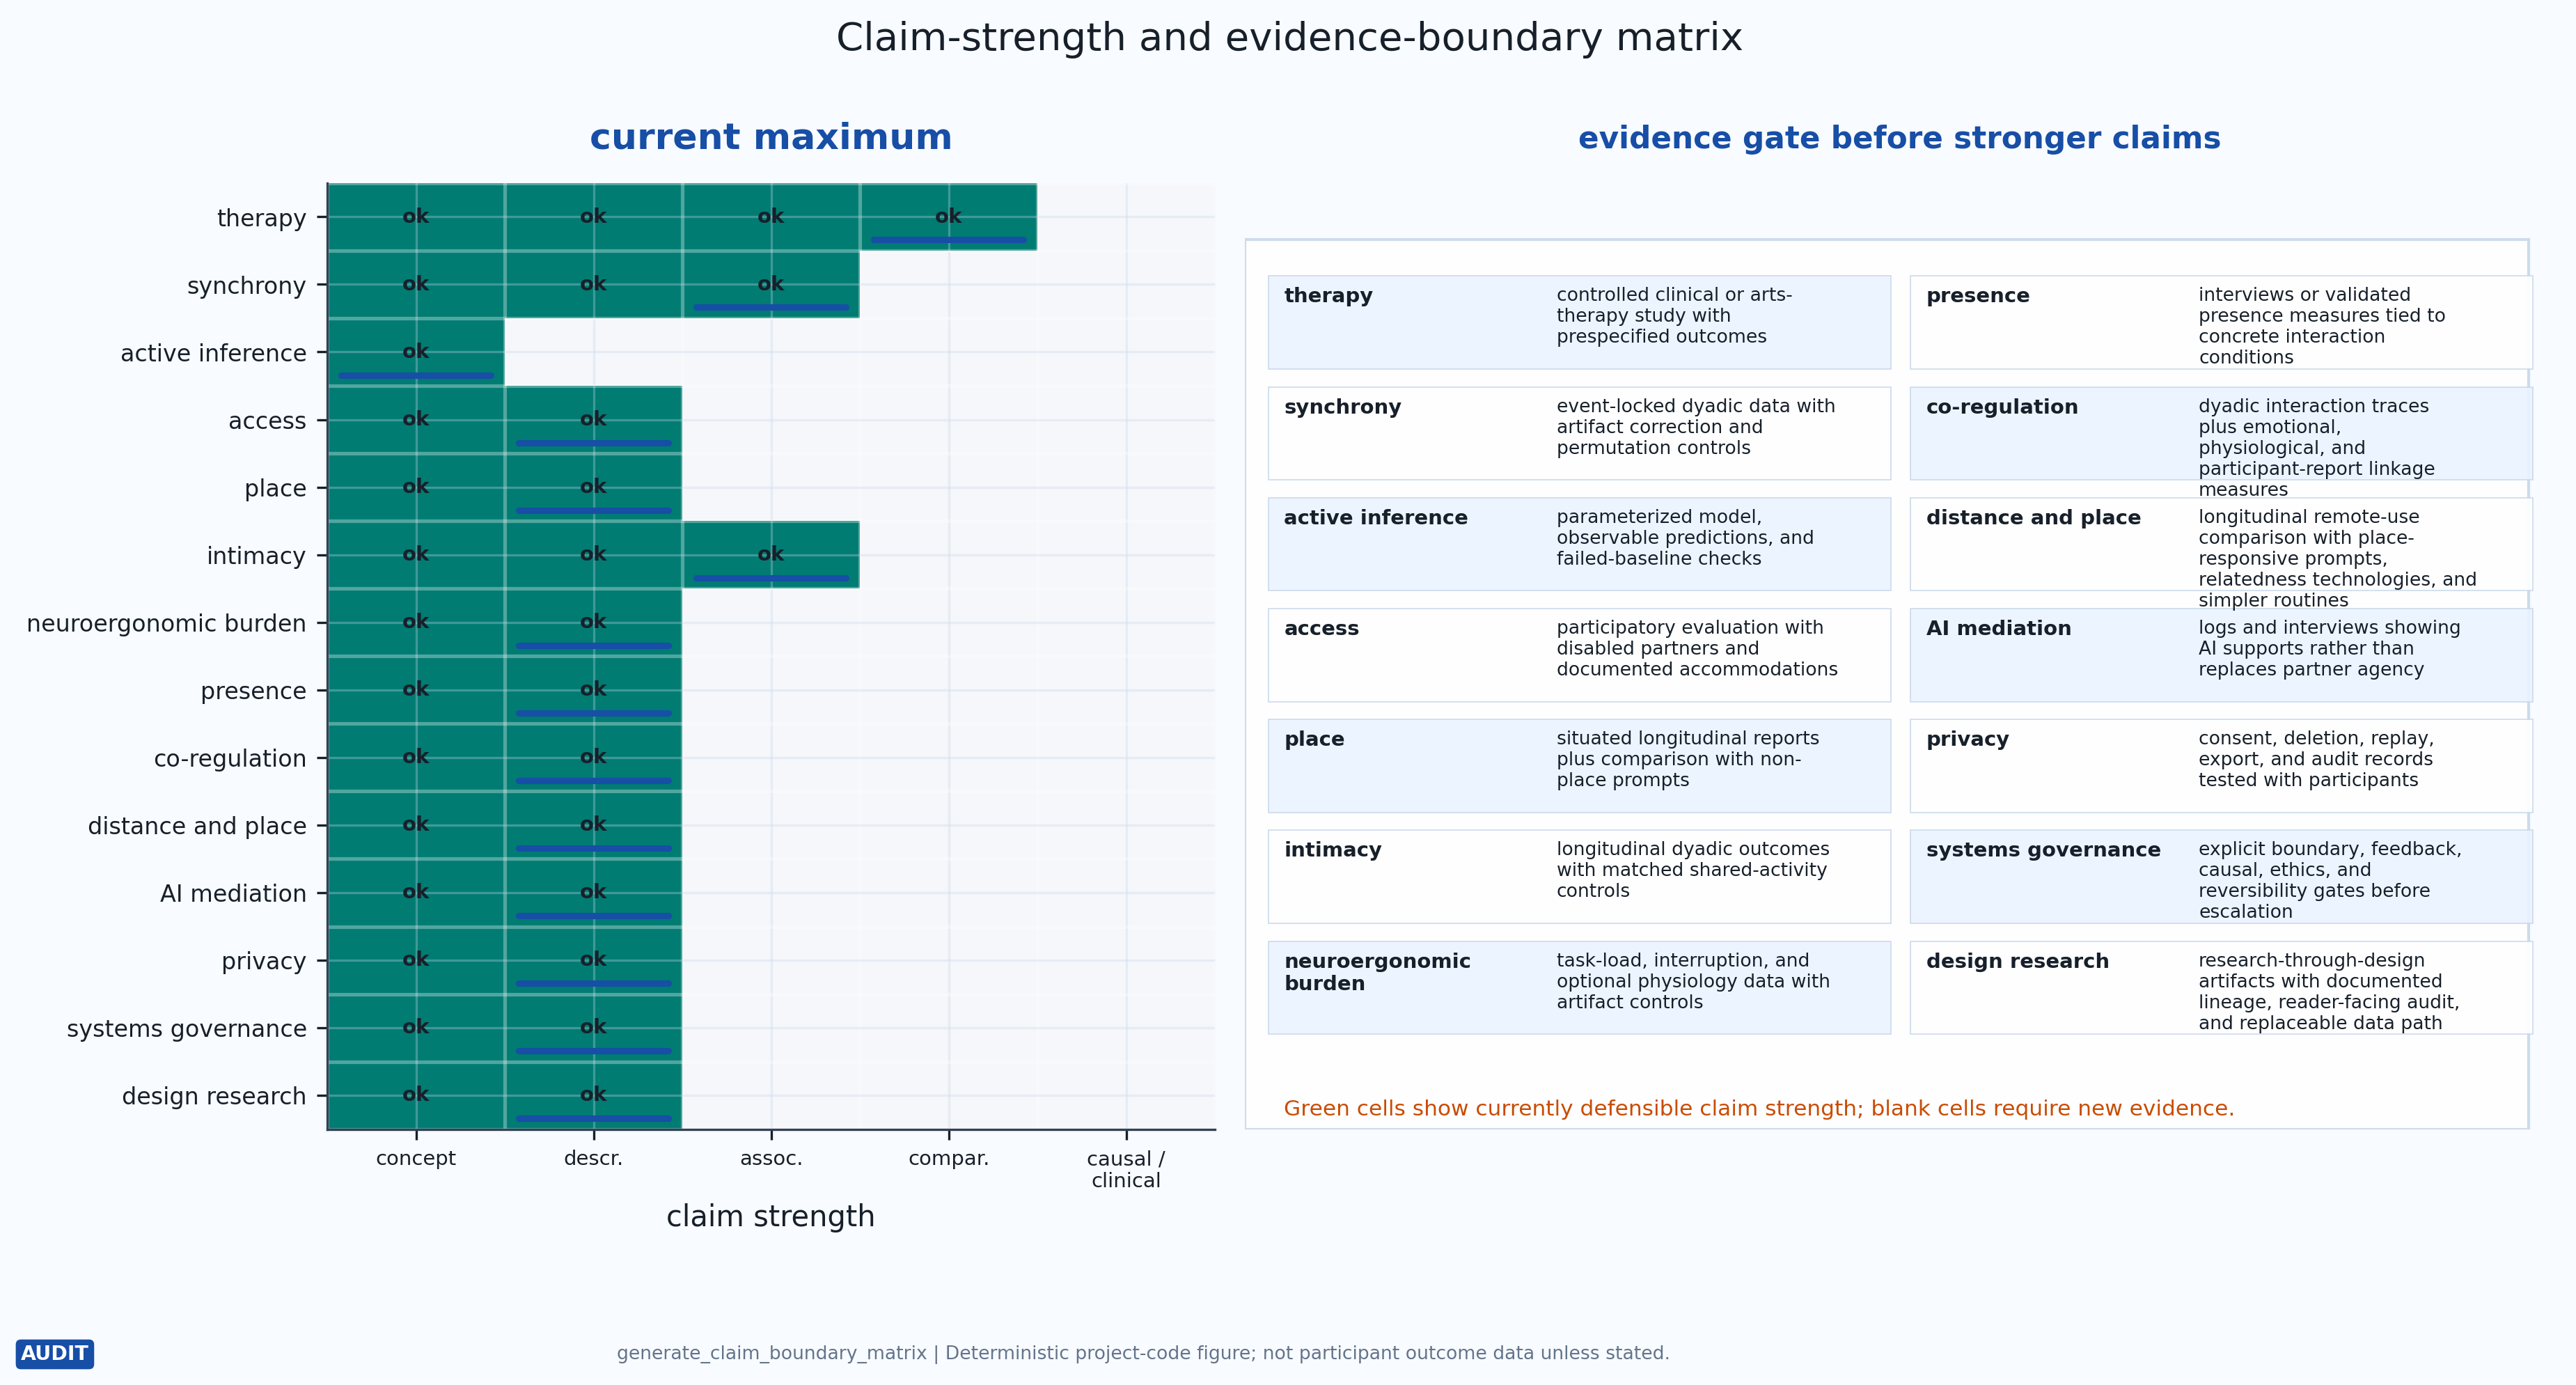
\includegraphics[width=0.9\linewidth,height=0.46\textheight,keepaspectratio,alt={Claim-strength and evidence-boundary matrix for DigiPPPiP. The matrix is generated by generate\_claim\_boundary\_matrix() from src/source\_quality.py; read rows as reviewer-risk domains, labelled green cells and blue rule marks as currently defensible claim levels, and the right panel as the evidence gate required for stronger language. It supports adversarial validity checking. The matrix is conceptual, and a domain can move only after direct study evidence is added.}]{../figures/claim_boundary_matrix.png}
\caption{Claim-strength and evidence-boundary matrix for DigiPPPiP. The
matrix is generated by
\protect\breaktt{generate\_claim\_boundary\_matrix()} from
\protect\breaktt{src/source\_quality.py}; read rows as reviewer-risk
domains, labelled green cells and blue rule marks as currently
defensible claim levels, and the right panel as the evidence gate
required for stronger language. It supports adversarial validity
checking. The matrix is conceptual, and a domain can move only after
direct study evidence is added.}\label{fig:claim_boundary_matrix}
\end{figure}

The boundary matrix is paired with a claim ledger rather than left as an
abstract warning. \breaktt{src/claim\_ledger.py} records recurring
manuscript claim families, their section, citekeys, present maximum
strength, and the evidence needed to upgrade them.
\breakseq{[@fig:claim\_ledger\_matrix]} makes the ledger visible. This also
documents the role of Perplexity and web search in the workflow:
discovery tools may nominate sources, but a citekey enters the ledger
only after the title, venue, year, and DOI or stable URL have been
checked against Crossref, a publisher page, an official standard, or an
archival record.

\begin{figure}
\centering
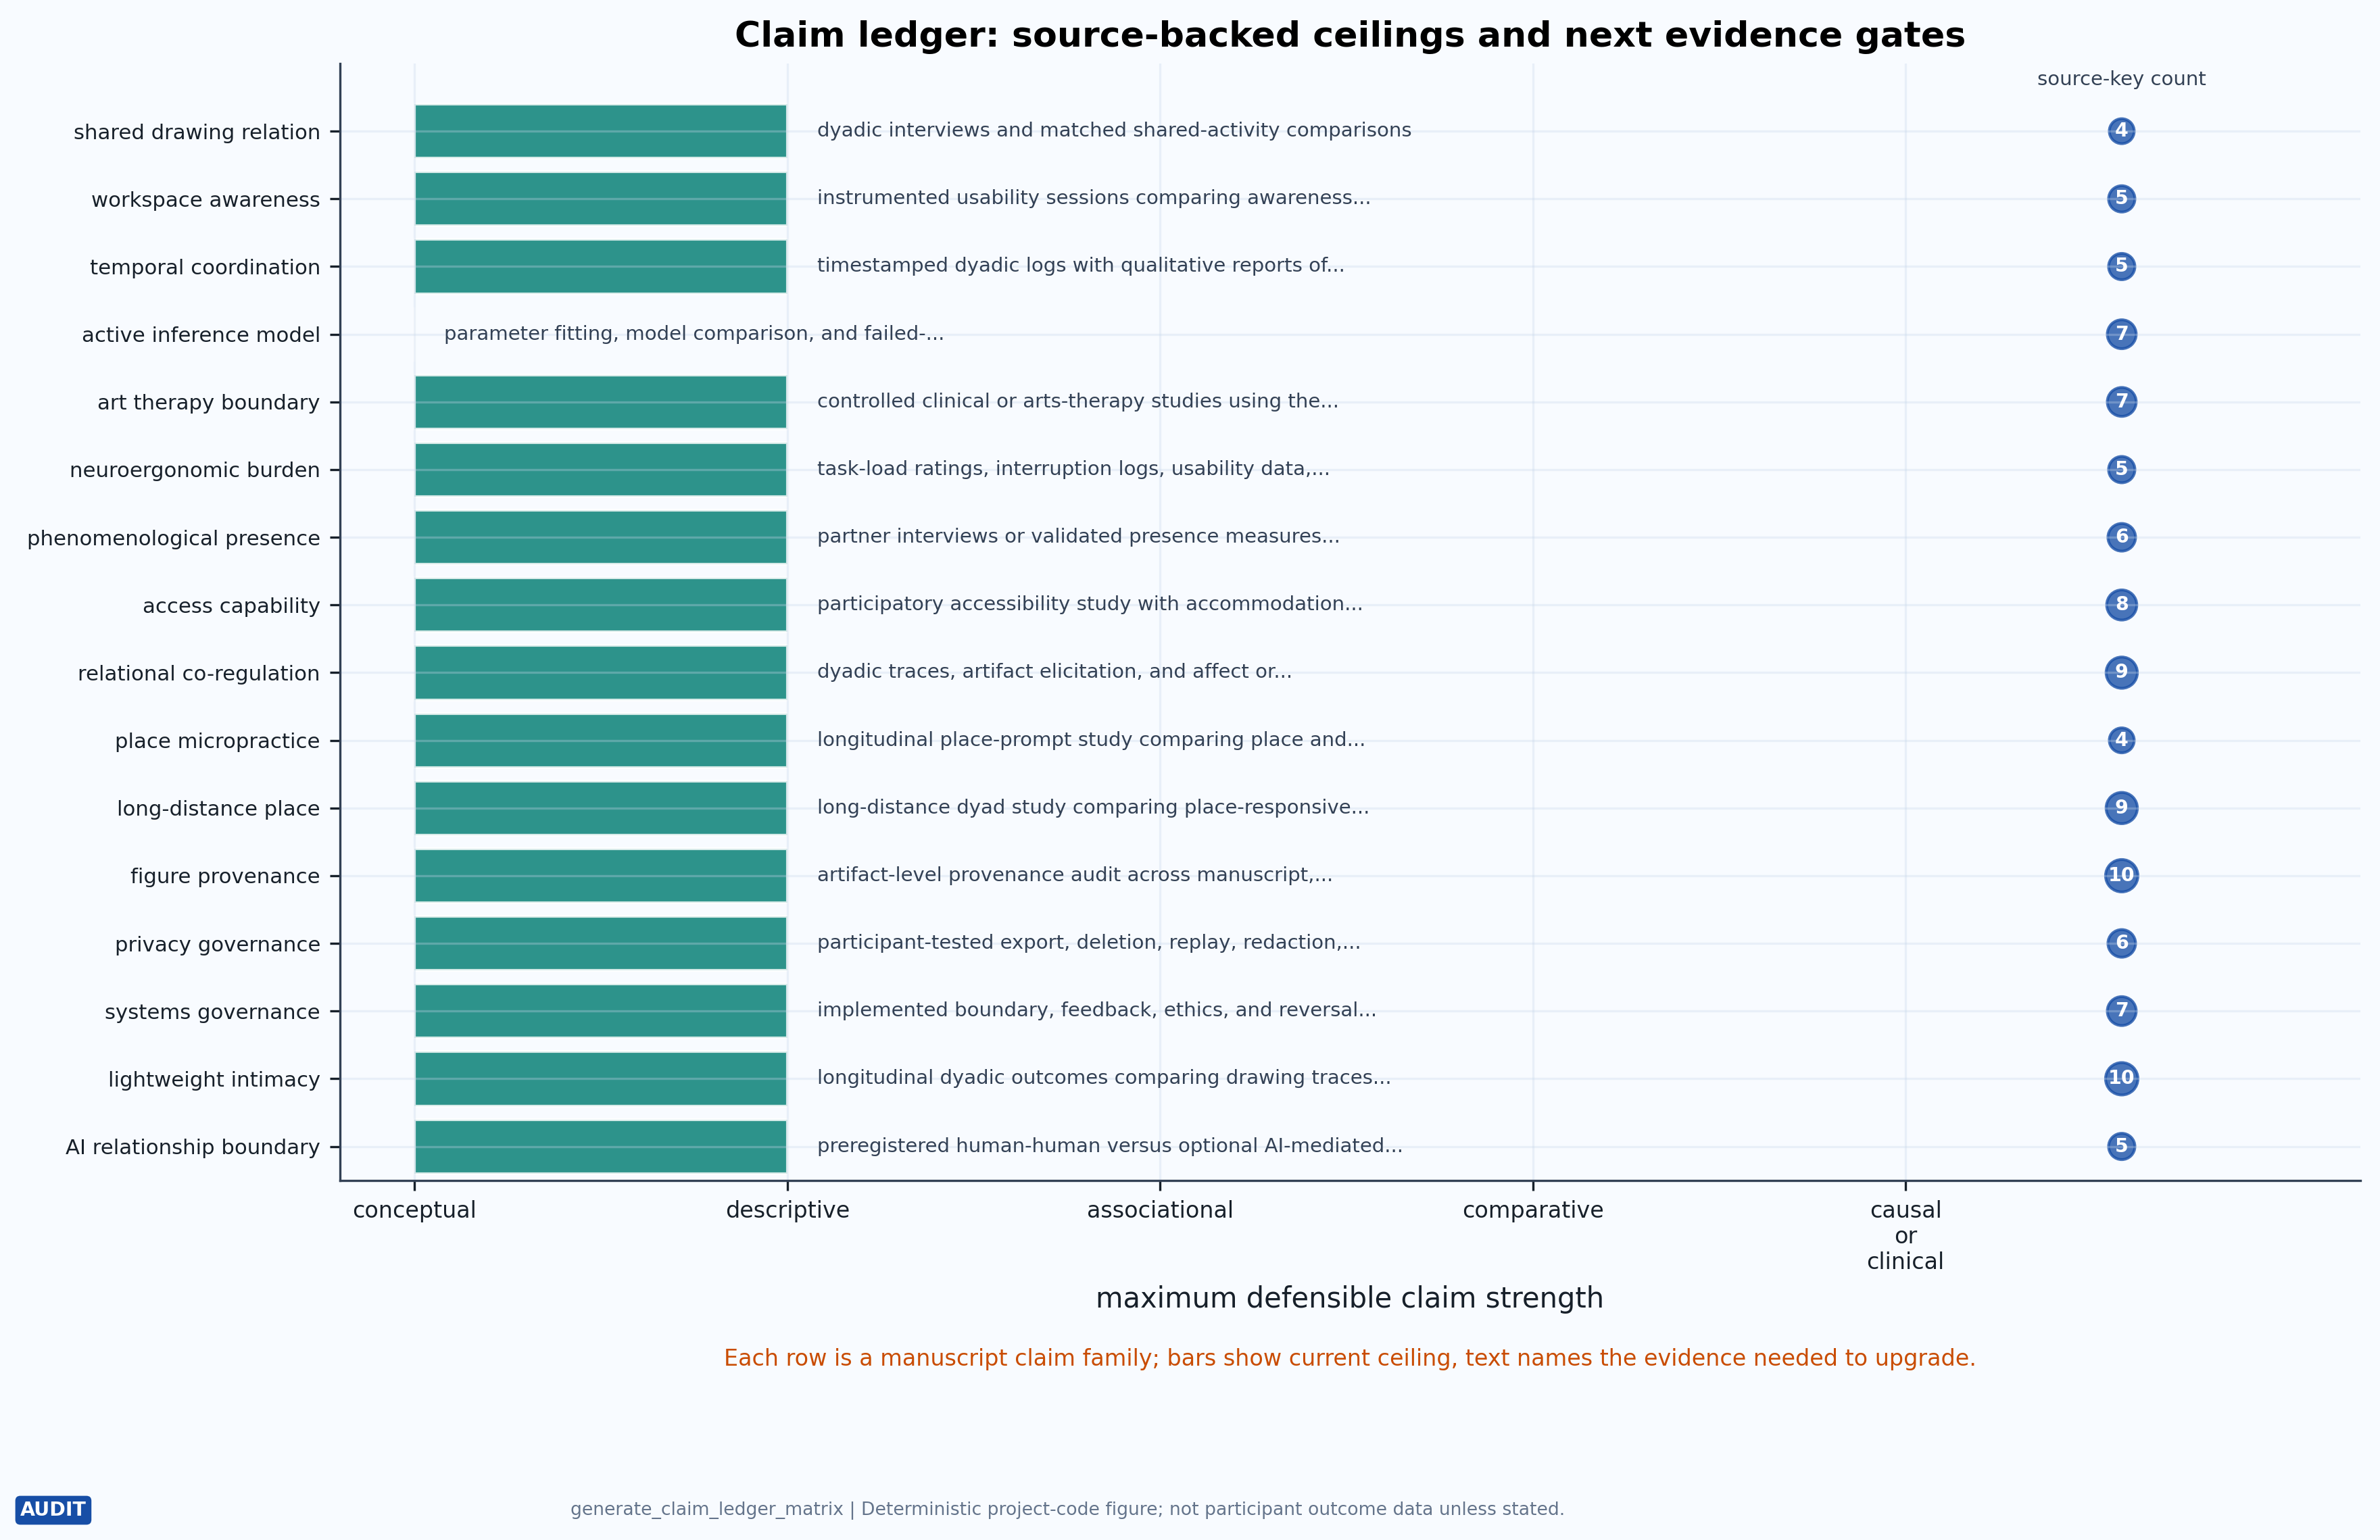
\includegraphics[width=0.9\linewidth,height=0.46\textheight,keepaspectratio,alt={Claim-ledger matrix linking manuscript claim families to evidence ceilings and upgrade gates. The figure is generated by generate\_claim\_ledger\_matrix() from src/claim\_ledger.py; read each row as a stable claim family, each bar as the current maximum claim strength, the blue numbered marker as evidence-key count, and the right-hand text as the next evidence gate. It supports source-to-claim governance rather than an empirical result. A stronger bar requires direct study evidence, not a more adjacent citation.}]{../figures/claim_ledger_matrix.png}
\caption{Claim-ledger matrix linking manuscript claim families to
evidence ceilings and upgrade gates. The figure is generated by
\protect\breaktt{generate\_claim\_ledger\_matrix()} from
\protect\breaktt{src/claim\_ledger.py}; read each row as a stable claim
family, each bar as the current maximum claim strength, the blue
numbered marker as evidence-key count, and the right-hand text as the
next evidence gate. It supports source-to-claim governance rather than
an empirical result. A stronger bar requires direct study evidence, not
a more adjacent citation.}\label{fig:claim_ledger_matrix}
\end{figure}

\breaktt{src/source\_verification.py} makes that rule executable. Each
governed citekey receives a locator, verification URL, checked-as-of
date, source tier, claim family, manuscript location, and recheck
trigger. The audit prioritizes 2024--2026 sources, preprints, AI claims,
digital-health claims, governance sources, and reporting standards for
refresh before submission. \breakseq{[@fig:source\_verification\_readiness]}
renders the current source-verification state from the same governed
citekey surfaces used by tests: claim ledger, evidence graph,
figure-method source bridge, and study-readiness cases. The ledger is
intentionally stricter than a bibliography because it asks what claim
family a source is allowed to support and when it must be rechecked.

\begin{figure}
\centering
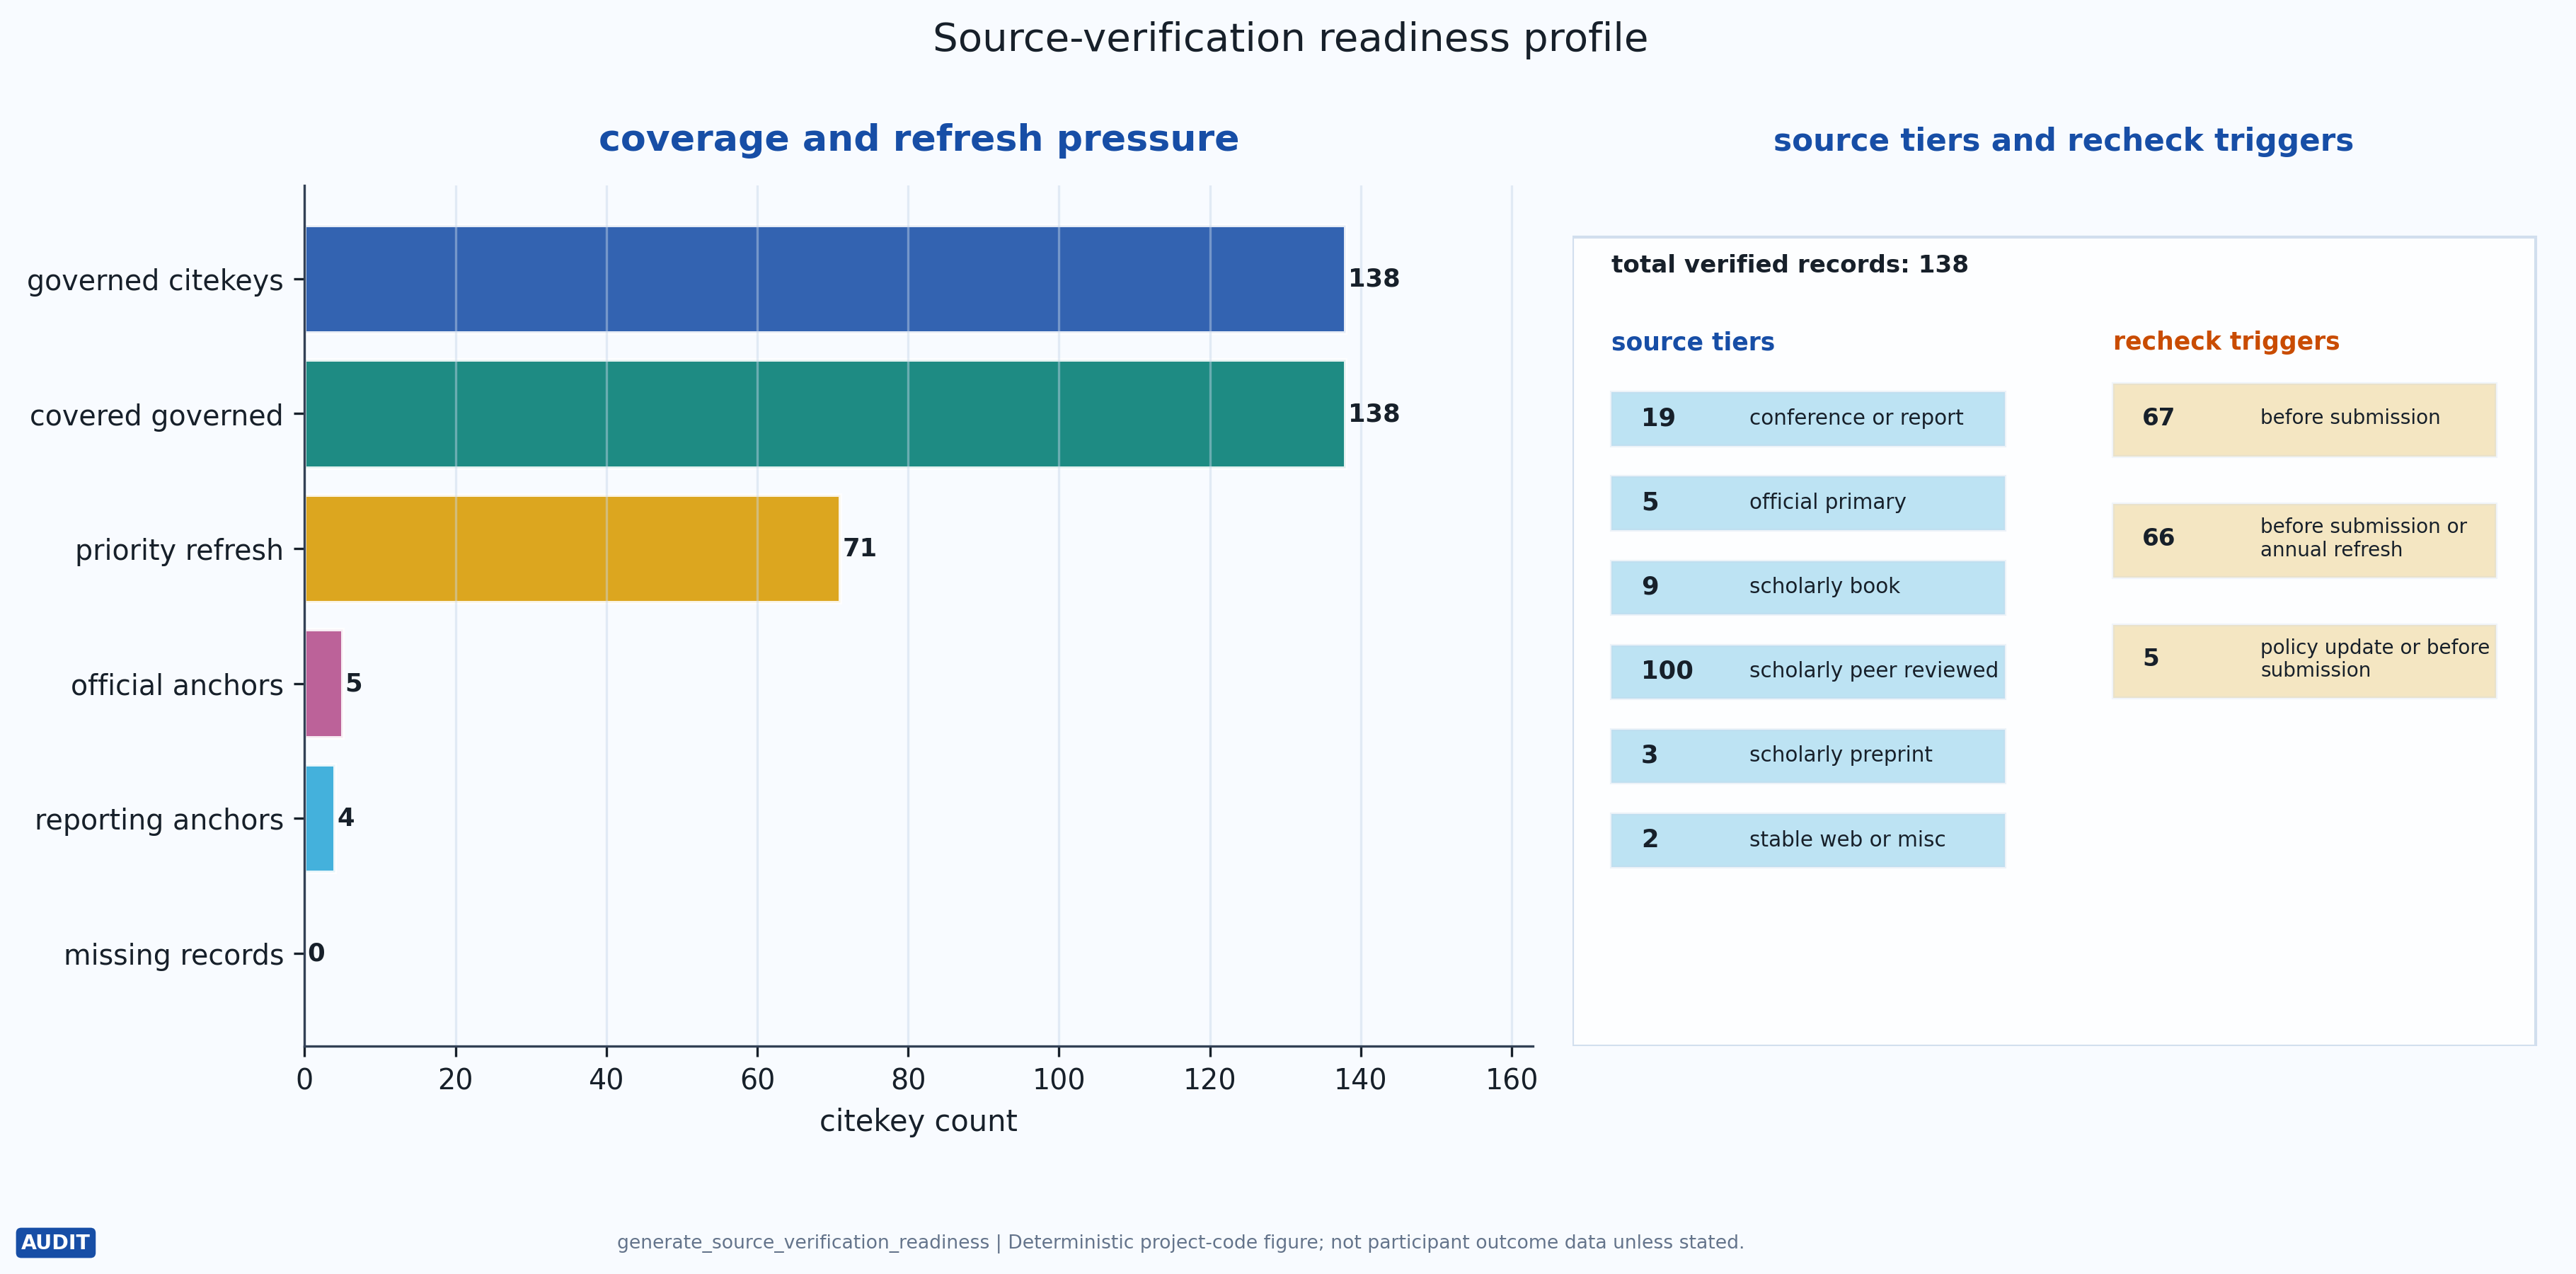
\includegraphics[width=0.95\linewidth,height=0.46\textheight,keepaspectratio,alt={Source-verification readiness profile for governed DigiPPPiP citekeys. The figure is generated by generate\_source\_verification\_readiness() from src/source\_verification.py; read the left panel as labelled citekey coverage and priority-refresh pressure, and the right panel as source-tier and recheck-trigger counts in audit cards. It supports provenance auditing rather than literature synthesis. A zero missing-record count means the ledger has locators and metadata, not that every source independently validates DigiPPPiP.}]{../figures/source_verification_readiness.png}
\caption{Source-verification readiness profile for governed DigiPPPiP
citekeys. The figure is generated by
\protect\breaktt{generate\_source\_verification\_readiness()} from
\protect\breaktt{src/source\_verification.py}; read the left panel as
labelled citekey coverage and priority-refresh pressure, and the right
panel as source-tier and recheck-trigger counts in audit cards. It
supports provenance auditing rather than literature synthesis. A zero
missing-record count means the ledger has locators and metadata, not
that every source independently validates
DigiPPPiP.}\label{fig:source_verification_readiness}
\end{figure}
\end{frame}

\begin{frame}[fragile,allowframebreaks]{Systems Boundary and Feedback
Governance}
\protect\phantomsection\label{systems-boundary-and-feedback-governance}
A first-principles pass reduces DigiPPPiP to a small hard kernel: two
human partners, perceivable marks, temporal structure, response
opportunity, and accountable persistence.
\breaktt{src/systems\_governance.py} makes the rest explicit as governed
branches rather than implicit scope creep. The current systems layer
records 6 boundary elements, 5 feedback loops, 5 causal assumptions, and
5 ethics gates, with a completeness score of 1. Active-inference and
enactive accounts support the action-perception framing and
Markov-blanket caution, while contextual privacy, values-in-design, and
human-subjects governance anchor the participant-facing side of the
boundary \breakseq{[@ramstead2020two; @nissenbaum2011contextualprivacy;
@shilton2012values; @hhs2025cfr46; @wma2024helsinki]}.

The boundary table keeps the human-human drawing loop inside the kernel
and marks event logs, place context, physiology, AI assistance, and
clinical translation as support structures or optional branches. Each
branch has a reversal gate: place prompts can be declined or coarsened;
physiology requires separate consent and artifact controls; AI
suggestions must be labelled, rejectable, undoable, and separable from
partner authorship; clinical translation stays out of scope until a
reviewed intervention protocol exists. This is a systems-governance
claim, not an efficacy claim. It says that the framework can name its
boundaries and stop conditions before it asks participants or reviewers
to trust them.

The feedback layer is deliberately adversarial. Action-perception loops
should preserve mutual agency; privacy loops should default to the
stricter dyadic archive choice; access loops should respond to fatigue,
sensory mismatch, and assistance needs; AI loops should detect
authorship confusion or partner substitution; evidence-escalation loops
should downgrade language when controls or participant reports do not
support a stronger claim. This makes falsification operational: if
matched controls explain the same relatedness reports, if place prompts
do not change situated memory, if replay feels like surveillance, if AI
reduces co-authorship, or if physiological linkage disappears after
artifact correction, the corresponding claim boundary narrows rather
than hardens.
\end{frame}

\begin{frame}[allowframebreaks]{Evidence Scope and Non-Claims}
\protect\phantomsection\label{evidence-scope-and-non-claims}
The present manuscript implements a design and governance architecture,
not a completed empirical evaluation. It demonstrates that DigiPPPiP
concepts can be expressed as manuscript sections, tested primitives,
generated figures, source ledgers, claim boundaries, protocol gates, and
render artifacts. It does not demonstrate therapeutic efficacy,
relationship improvement, neural coupling, universal accessibility, or
AI benefit. Active inference, geometric hyperscanning, narrative
information, and outcome modeling are used as modeling and measurement
lenses; they become mechanisms only if future studies fit them to
observed sessions, compare them with plausible alternatives, and survive
the falsifiers named in the protocol.

This scope statement also governs visual interpretation. Architecture
figures show boundaries, not deployed software. Data-flow figures show
what a study should record, not what participants have already produced.
Simulation plots show toy diagnostics, not human behavior. Audit figures
show that the manuscript has local governance machinery, not that
DigiPPPiP is externally validated. Those distinctions are intentionally
repetitive because they are the main defense against attractive diagrams
becoming overclaims.
\end{frame}

\begin{frame}[fragile,allowframebreaks]{Interactive Web Instantiation
(Conceptual Demo)}
\protect\phantomsection\label{interactive-web-instantiation-conceptual-demo}
DigiPPPiP is also implemented as a small, self-contained interactive web
canvas so that the cyberphysical argument in \breakseq{[@sec:cyberphysical]} is
concrete rather than diagrammatic only. The application pairs people on
a shared, low-latency drawing surface and relays strokes, undos, and
cursor positions through a Socket.IO server; each participant is
identified by a lightweight Adjective-Fruit moniker that follows their
cursor across the shared field. Its design kernel is deliberately the
minimum viable kernel described in \breakseq{[@sec:cyberphysical]}: partners, a
shared mark field, perceptible traces of agency, and consentful control
over persistence. The running tool is therefore a working instantiation
of the architecture in \breakseq{[@fig:cpss\_architecture]} rather than a
clinical instrument.

\begin{figure}
\centering
\includegraphics[width=0.95\linewidth,height=0.46\textheight,keepaspectratio,alt={The running Digi-PPPiP web canvas in its default dark theme, showing freehand strokes, the active-user moniker (Cozy Kiwi), the waiting-for-partner status, the drawing palette, and the simulated Coupled Dynamics panel. Captured from the running Vite/Socket.IO demo stack by generate\_webapp\_main\_canvas(); read the canvas as the shared mark field, the top bar as session state, and the bottom-right panel as the computed modeling lens. It supports the methods argument that the cyberphysical substrate in \breakseq{[@fig:cpss\_architecture]} is implementable. The screenshot is conceptual; assessed usability and relational effects would require the study protocol in \breakseq{[@sec:methods\_protocol]}.}]{../figures/webapp_main_canvas.png}
\caption{The running Digi-PPPiP web canvas in its default dark theme,
showing freehand strokes, the active-user moniker (Cozy Kiwi), the
waiting-for-partner status, the drawing palette, and the simulated
Coupled Dynamics panel. Captured from the running Vite/Socket.IO demo
stack by \protect\breaktt{generate\_webapp\_main\_canvas()}; read the
canvas as the shared mark field, the top bar as session state, and the
bottom-right panel as the computed modeling lens. It supports the
methods argument that the cyberphysical substrate in
\breakseq{[@fig:cpss\_architecture]} is implementable. The screenshot is
conceptual; assessed usability and relational effects would require the
study protocol in
\breakseq{[@sec:methods\_protocol]}.}\label{fig:webapp_main_canvas}
\end{figure}

The screen captures deliberately confine the relational claim.
\breakseq{[@fig:webapp\_main\_canvas]} shows a single-user session; the paired
dynamics the framework theorizes are rendered only as simulated values.
\breakseq{[@fig:webapp\_metrics\_dashboard]} isolates the live dashboard, where
Variational Free Energy, Inter-Brain Synchrony, and Narrative Entropy
are displayed with an explicit simulated-illustrative-values disclaimer.
These numbers are generated client-side as a demonstration of the
modeling lens; they are not experimental measurements and must not be
read as evidence of neural coupling or therapeutic effect.

\begin{figure}
\centering
\includegraphics[width=0.6\linewidth,height=0.46\textheight,keepaspectratio,alt={The Coupled Dynamics dashboard as rendered in the live app, isolating the simulated Variational Free Energy, Inter-Brain Synchrony, and Narrative Entropy readouts and their progress bars. Captured by generate\_webapp\_metrics\_dashboard(); read each row as metric label, value, and relative magnitude. It supports the protocol distinction between a computed modeling lens and an outcome measurement. The values are simulated and illustrative; real values would require physiological instrumentation and the consent and logging gates in \breakseq{[@sec:methods\_protocol]}.}]{../figures/webapp_metrics_dashboard.png}
\caption{The Coupled Dynamics dashboard as rendered in the live app,
isolating the simulated Variational Free Energy, Inter-Brain Synchrony,
and Narrative Entropy readouts and their progress bars. Captured by
\protect\breaktt{generate\_webapp\_metrics\_dashboard()}; read each row
as metric label, value, and relative magnitude. It supports the protocol
distinction between a computed modeling lens and an outcome measurement.
The values are simulated and illustrative; real values would require
physiological instrumentation and the consent and logging gates in
\breakseq{[@sec:methods\_protocol]}.}\label{fig:webapp_metrics_dashboard}
\end{figure}

The interface also exposes configuration choices that matter for the
accessibility and privacy commitments in \breakseq{[@sec:accessibility]}.
\breakseq{[@fig:webapp\_light\_theme]} shows the same canvas in a light theme,
and \breakseq{[@fig:webapp\_theme\_settings]} shows the theme and
canvas-background settings against a plain white canvas. These options
are not cosmetic polish; they operationalize the ability-based and
WCAG-informed design commitments of the framework by letting a pair
choose contrast and background settings that fit their access needs,
while session and archive controls remain distinct from the visible
drawing surface.

\begin{figure}
\centering
\includegraphics[width=0.9\linewidth,height=0.46\textheight,keepaspectratio,alt={The same Digi-PPPiP canvas switched to the light theme. Captured by generate\_webapp\_light\_theme(); read it as the tool's visual-contrast alternative to \breakseq{[@fig:webapp\_main\_canvas]}. It supports the accessibility commitment that theme and contrast are user-selectable. The screenshot is conceptual; demonstrated accessibility benefit would require an accessibility audit such as \breakseq{[@fig:accessibility\_audit\_radar]}.}]{../figures/webapp_light_theme.png}
\caption{The same Digi-PPPiP canvas switched to the light theme.
Captured by \protect\breaktt{generate\_webapp\_light\_theme()}; read it
as the tool's visual-contrast alternative to
\breakseq{[@fig:webapp\_main\_canvas]}. It supports the accessibility
commitment that theme and contrast are user-selectable. The screenshot
is conceptual; demonstrated accessibility benefit would require an
accessibility audit such as
\breakseq{[@fig:accessibility\_audit\_radar]}.}\label{fig:webapp_light_theme}
\end{figure}

\begin{figure}
\centering
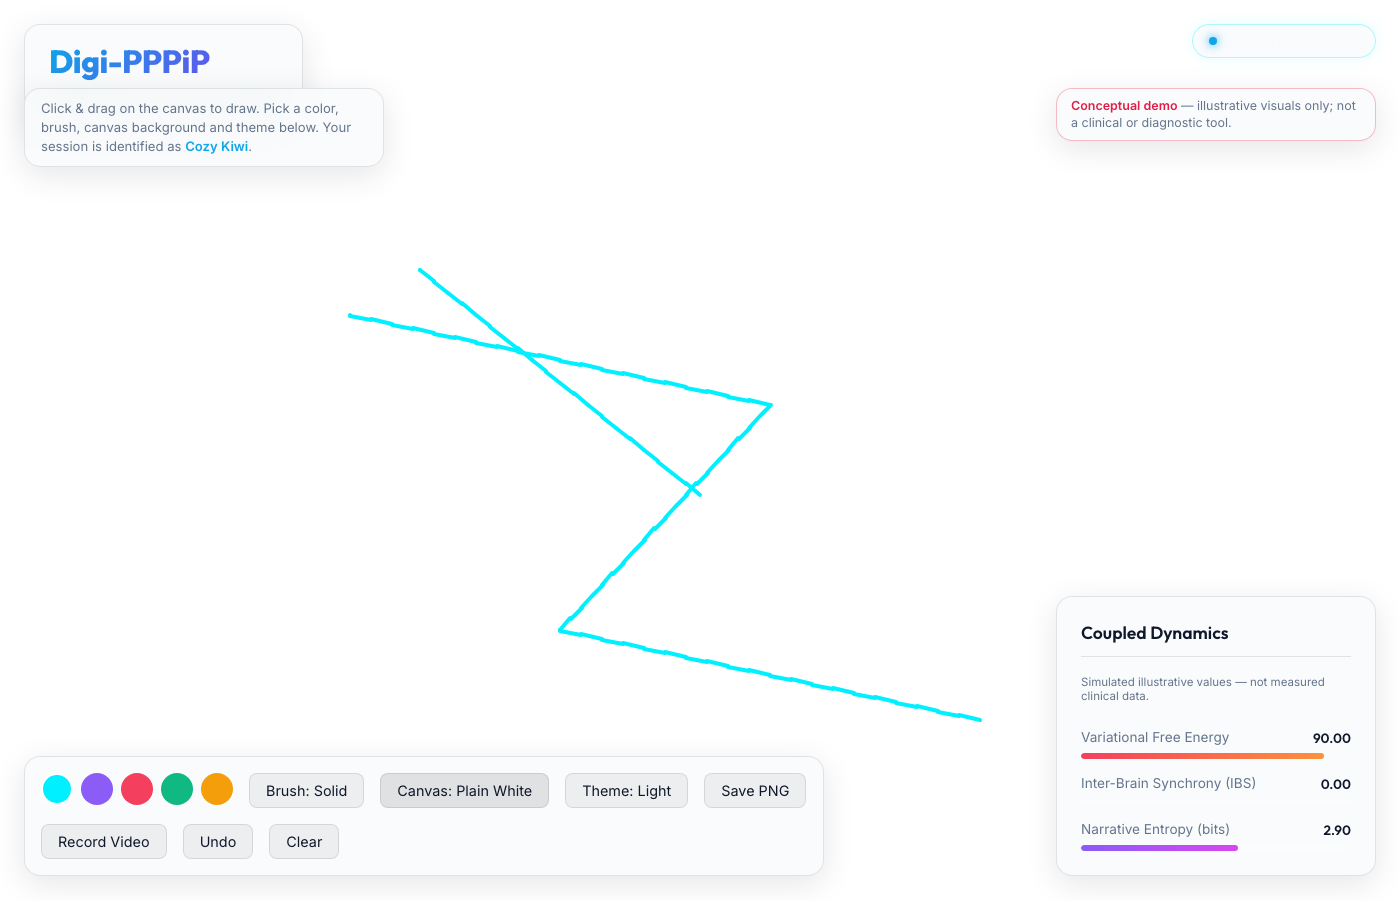
\includegraphics[width=0.9\linewidth,height=0.46\textheight,keepaspectratio,alt={Theme and canvas-background settings shown in the light theme against a plain white canvas. Captured by generate\_webapp\_theme\_settings(); read the control row as the selectable theme, brush, and background configuration. It supports the design-commitment argument that visual-contrast and background choices are first-order, user-facing settings. The screenshot is conceptual and shows interface configuration, not measured accessibility outcomes.}]{../figures/webapp_theme_settings.png}
\caption{Theme and canvas-background settings shown in the light theme
against a plain white canvas. Captured by
\protect\breaktt{generate\_webapp\_theme\_settings()}; read the control
row as the selectable theme, brush, and background configuration. It
supports the design-commitment argument that visual-contrast and
background choices are first-order, user-facing settings. The screenshot
is conceptual and shows interface configuration, not measured
accessibility outcomes.}\label{fig:webapp_theme_settings}
\end{figure}
\end{frame}

\begin{frame}[fragile,allowframebreaks]{Reproducible Figure Methods}
\protect\phantomsection\label{reproducible-figure-methods}
The figure-generation method is also part of the research protocol
rather than a cosmetic afterthought. Visualization grammars clarify how
data, marks, scales, and layers compose \breakseq{[@wilkinson2005grammar;
@wickham2010layered; @bostock2011d3; @satyanarayan2017vegalite]}, while
graphical-perception, color-use, and validation work shows that
scientific figures need perceptual, task, and design justification
rather than merely attractive styling \breakseq{[@cleveland1984graphical;
@munzner2009nested; @crameri2020colour]}. DigiPPPiP therefore treats
each generated figure as a small reproducible claim object: a scoped
argument, a method-lineage warrant, a tested primitive or explicitly
conceptual source, a visual encoding grammar, an aesthetic/accessibility
rule, a deterministic render, a registry entry, a caption contract, an
accessibility description, and a render validation gate.
\breakseq{[@fig:figure\_generation\_pipeline]} encodes that artifact chain. The
implemented method has 9 generation stages, 7 semantic encoding roles, 5
source-method families, 13 audit criteria, 8 required caption elements,
and a method-contract score of 1. The relevant scholarship supports this
restraint: effective figures need explicit design choices and accessible
description, visualization provenance should preserve why analytic
artifacts were produced, remote-health-monitoring visualization studies
should account for clinician comprehension and stakeholder-specific
granularity, interactive visual systems need inspectable operations,
accessible visualizations need navigable structure and custom reading
sequences, image-alt decisions need context-specific text alternatives,
and reproducible computational work needs organized, regenerable
artifacts \breakseq{[@kelleher2011guidelines; @rougier2014figures;
@ragan2016provenance; @lebaron2025remoteviz; @heer2012interactive;
@elavsky2024datanavigator; @jones2024customization;
@w3c2024altdecisiontree; @wilson2017goodenough; @rule2019jupyter;
@stodden2014reproducible; @lundgard2022accessible]}.

\begin{figure}
\centering
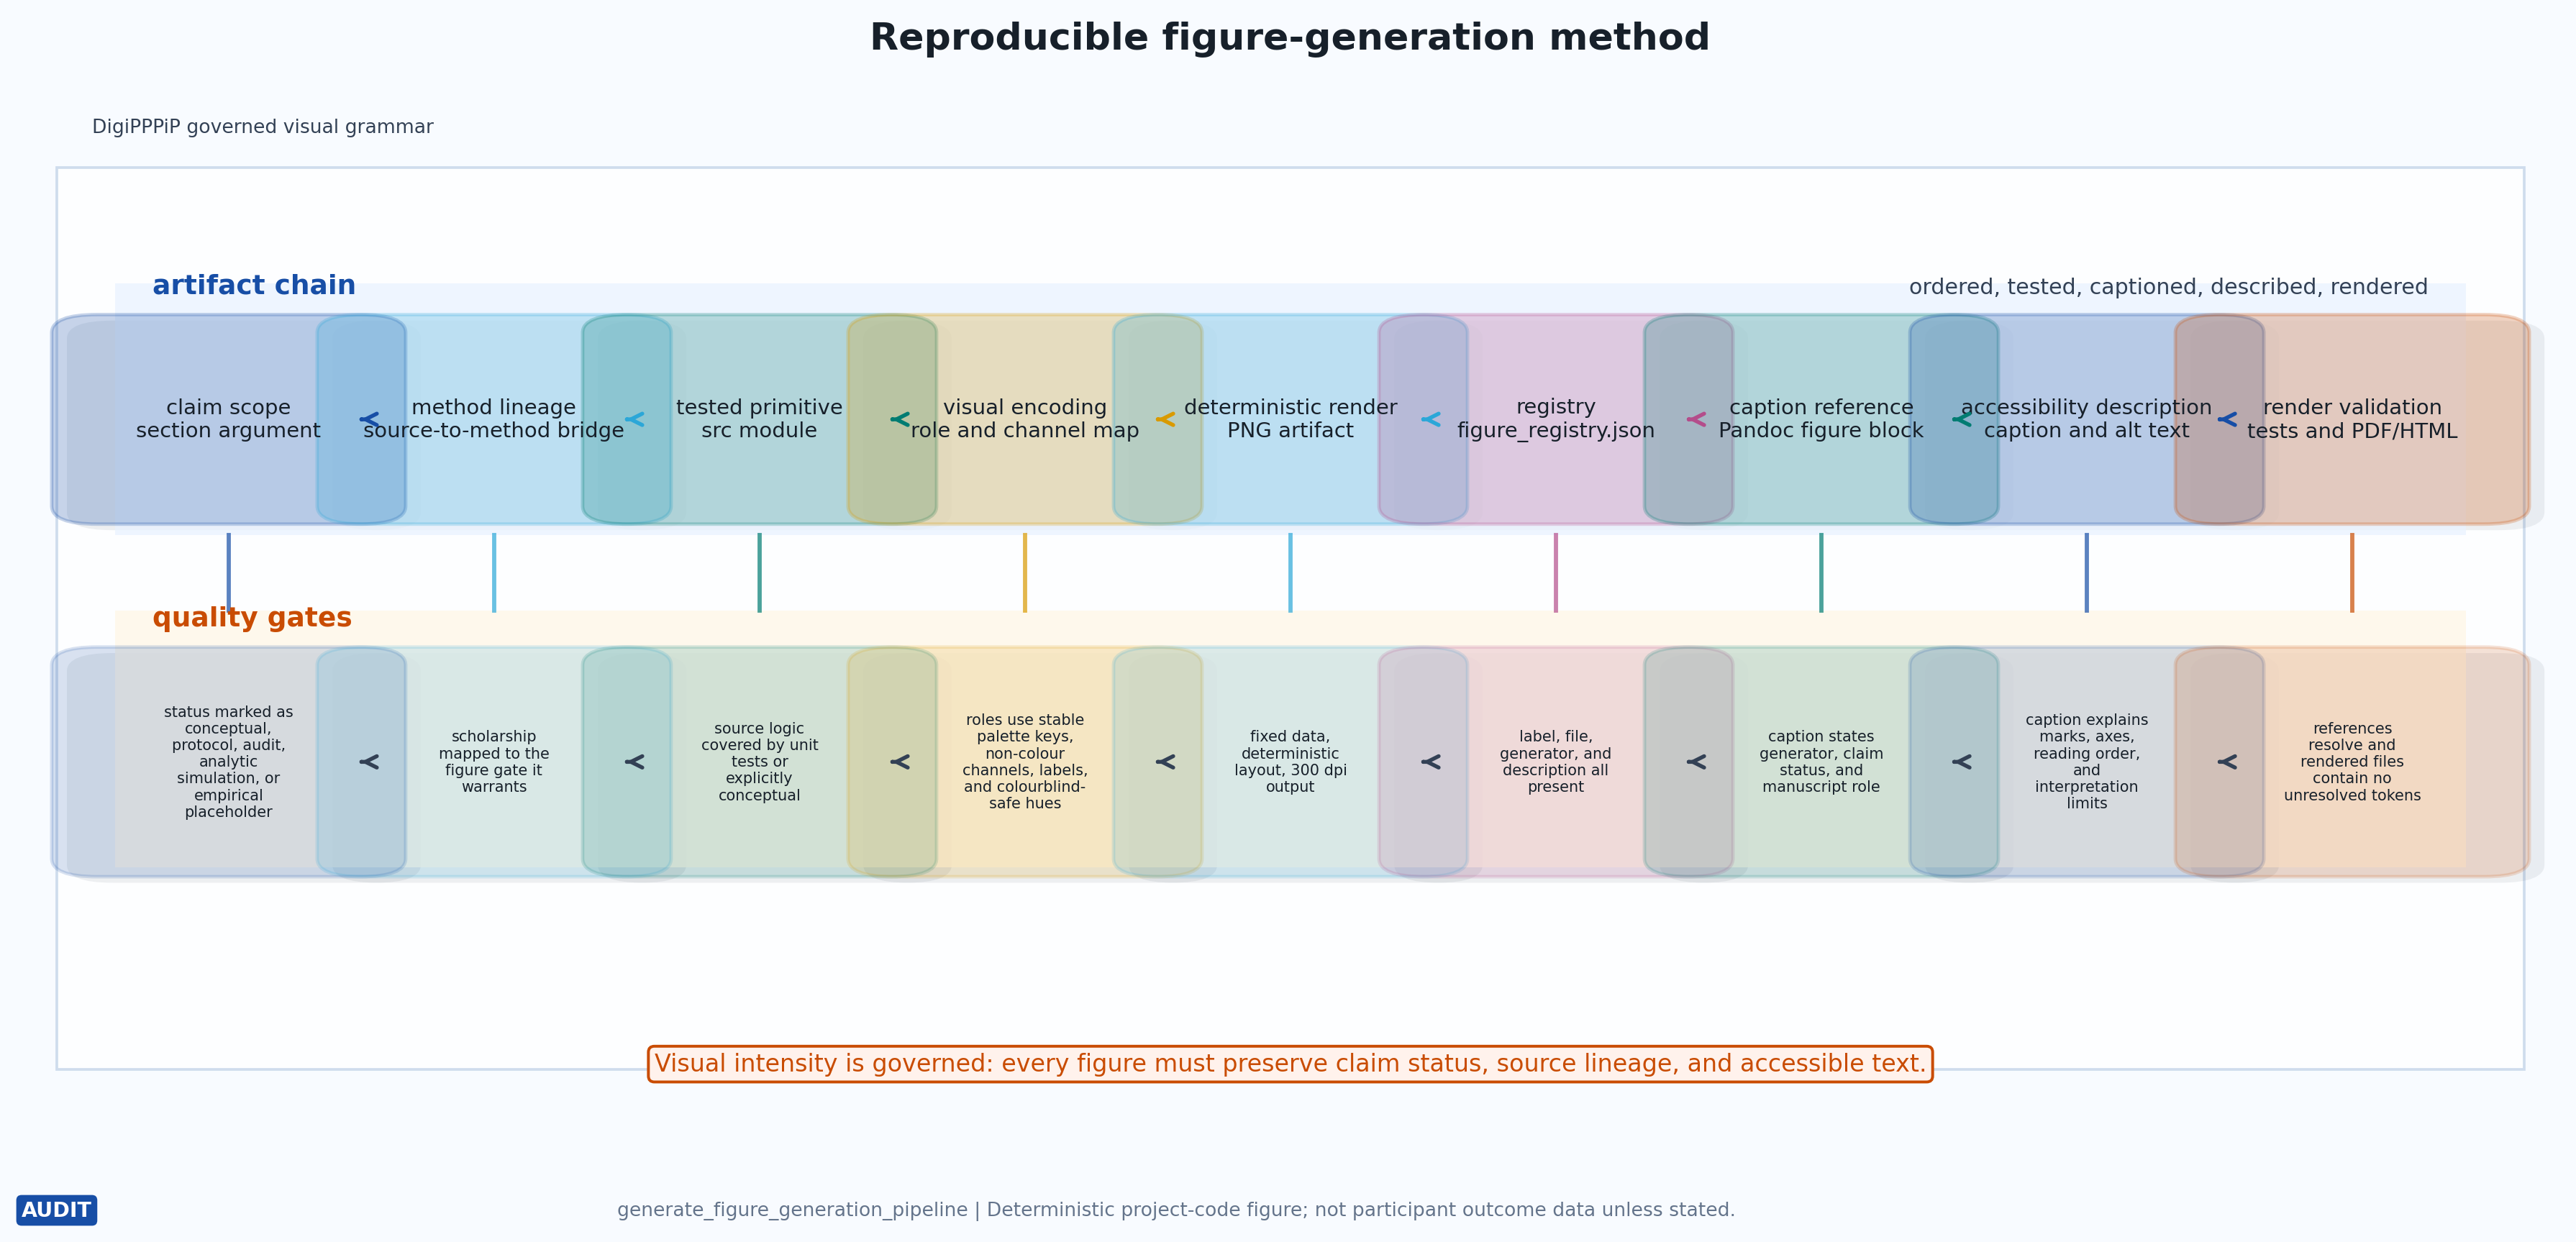
\includegraphics[width=0.95\linewidth,height=0.46\textheight,keepaspectratio,alt={Reproducible figure-generation method for DigiPPPiP. The pipeline is generated by generate\_figure\_generation\_pipeline() from src/figure\_methods.py; read the upper row as artifacts, the lower row as quality gates, and the colored lanes as the governed movement from scoped claim through accessibility description and render validation. It supports the methods argument that figures are reproducible claim objects. The pipeline is analytic, and future empirical figures should inherit the same gates.}]{../figures/figure_generation_pipeline.png}
\caption{Reproducible figure-generation method for DigiPPPiP. The
pipeline is generated by
\protect\breaktt{generate\_figure\_generation\_pipeline()} from
\protect\breaktt{src/figure\_methods.py}; read the upper row as
artifacts, the lower row as quality gates, and the colored lanes as the
governed movement from scoped claim through accessibility description
and render validation. It supports the methods argument that figures are
reproducible claim objects. The pipeline is analytic, and future
empirical figures should inherit the same
gates.}\label{fig:figure_generation_pipeline}
\end{figure}

Research-through-design scholarship explains why this workflow is not
merely a publishing convenience. HCI research-through-design treats
artifact making as a legitimate way to produce interaction-design
knowledge when the artifact, process, and contribution are made legible
\breakseq{[@zimmerman2007rtd; @gaver2012expectrtd]}. Annotated portfolios and
reflective design documentation make the same requirement more concrete:
design artifacts need comparative framing, annotations, and traces of
decision-making if they are to function as research outputs rather than
illustrations \breakseq{[@gaver2012annotated; @dalsgaard2012documentation]}.
DigiPPPiP applies that discipline to generated figures.
\breakseq{[@fig:method\_source\_bridge]} renders the source-to-method bridge. A
diagram is allowed to contribute conceptual structure only when its
method lineage, code path, registry row, caption, and claim boundary are
visible.

\begin{figure}
\centering
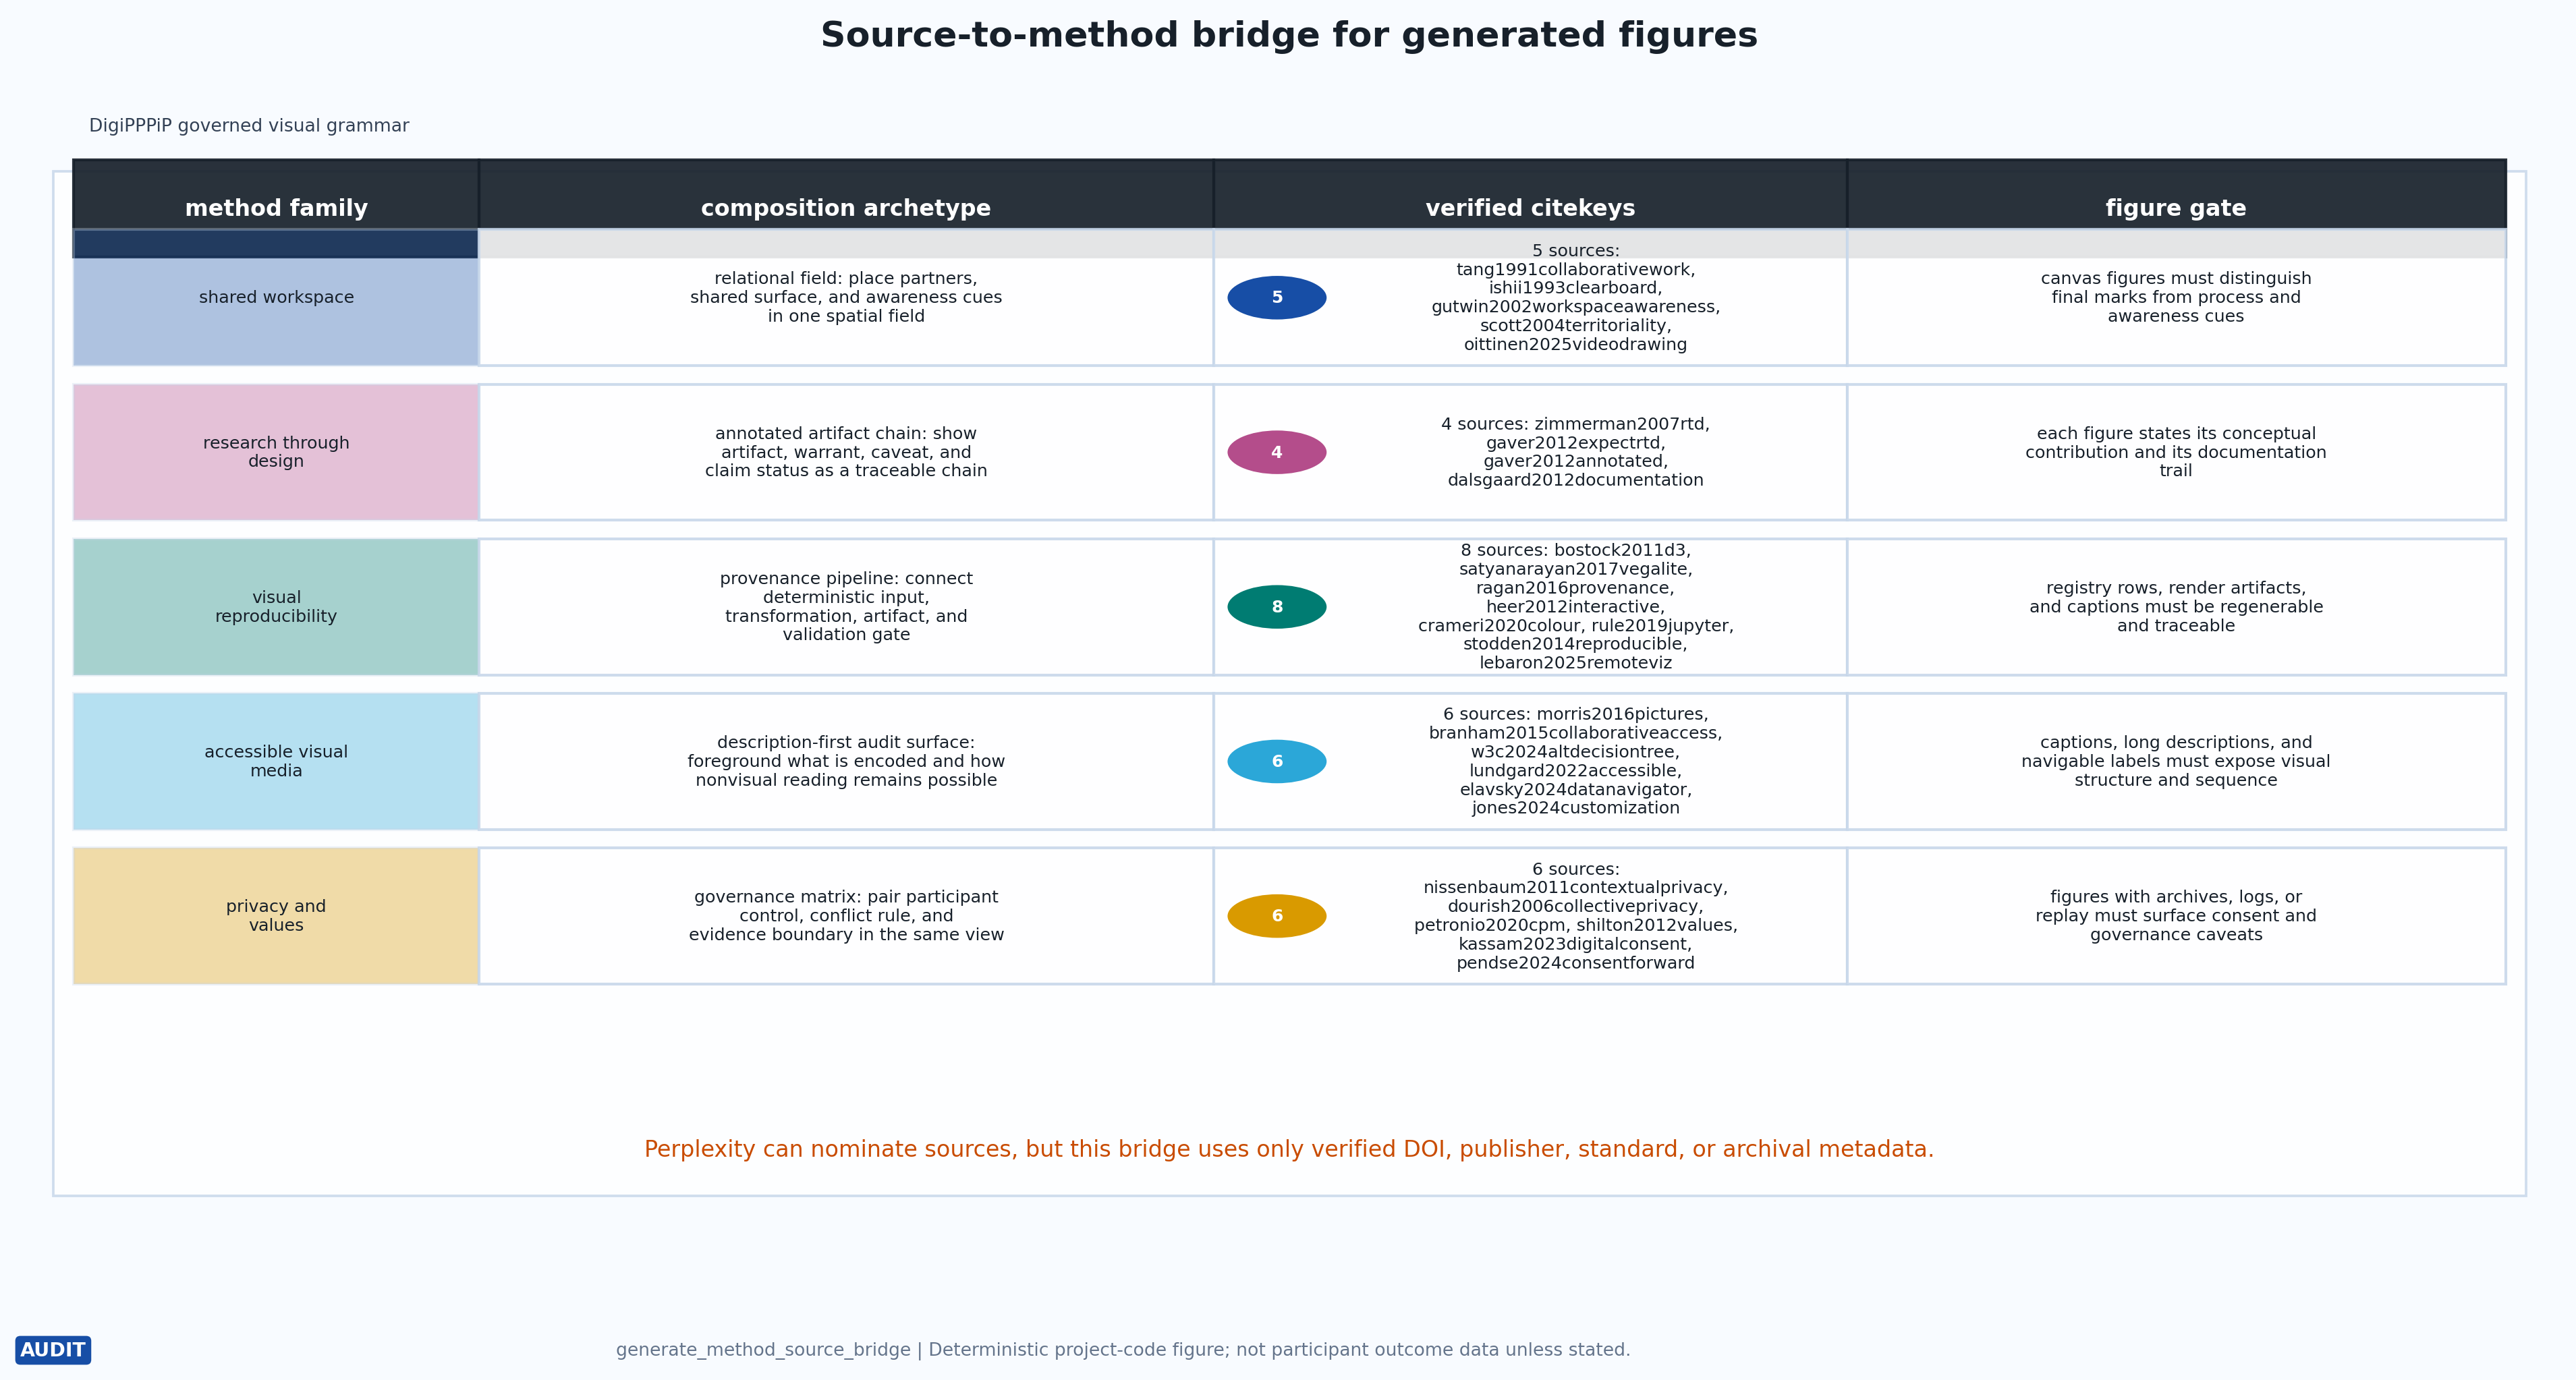
\includegraphics[width=0.95\linewidth,height=0.46\textheight,keepaspectratio,alt={Source-to-method bridge for generated DigiPPPiP figures. The figure is generated by generate\_method\_source\_bridge() from src/figure\_methods.py; read each row as a verified scholarly family, its composition archetype, the citekeys used by the project, source-count badges, and the gate it imposes on generated figures. It supports the methods claim that diagrams are research artifacts only when their warrant is traceable. The bridge is an audit device and does not turn conceptual figures into empirical evidence.}]{../figures/method_source_bridge.png}
\caption{Source-to-method bridge for generated DigiPPPiP figures. The
figure is generated by
\protect\breaktt{generate\_method\_source\_bridge()} from
\protect\breaktt{src/figure\_methods.py}; read each row as a verified
scholarly family, its composition archetype, the citekeys used by the
project, source-count badges, and the gate it imposes on generated
figures. It supports the methods claim that diagrams are research
artifacts only when their warrant is traceable. The bridge is an audit
device and does not turn conceptual figures into empirical
evidence.}\label{fig:method_source_bridge}
\end{figure}

\breakseq{[@fig:visual\_encoding\_matrix]} makes the visual grammar explicit.
Actors, artifacts, signals, contexts, evidence, models, and caveats are
assigned stable palette keys, non-color channels, hierarchy rules, and
accessibility constraints so that repeated figures can be interpreted as
a family without depending on hue alone. The grammar is intentionally
conservative: it separates human actors from software assistance, shared
artifacts from outcomes, signal traces from interpretation, and
placemaking contexts from universal community-scale claims. This makes
captions more auditable because the reader can compare the figure's
visual roles with the claim boundary that the prose asserts.

\begin{figure}
\centering
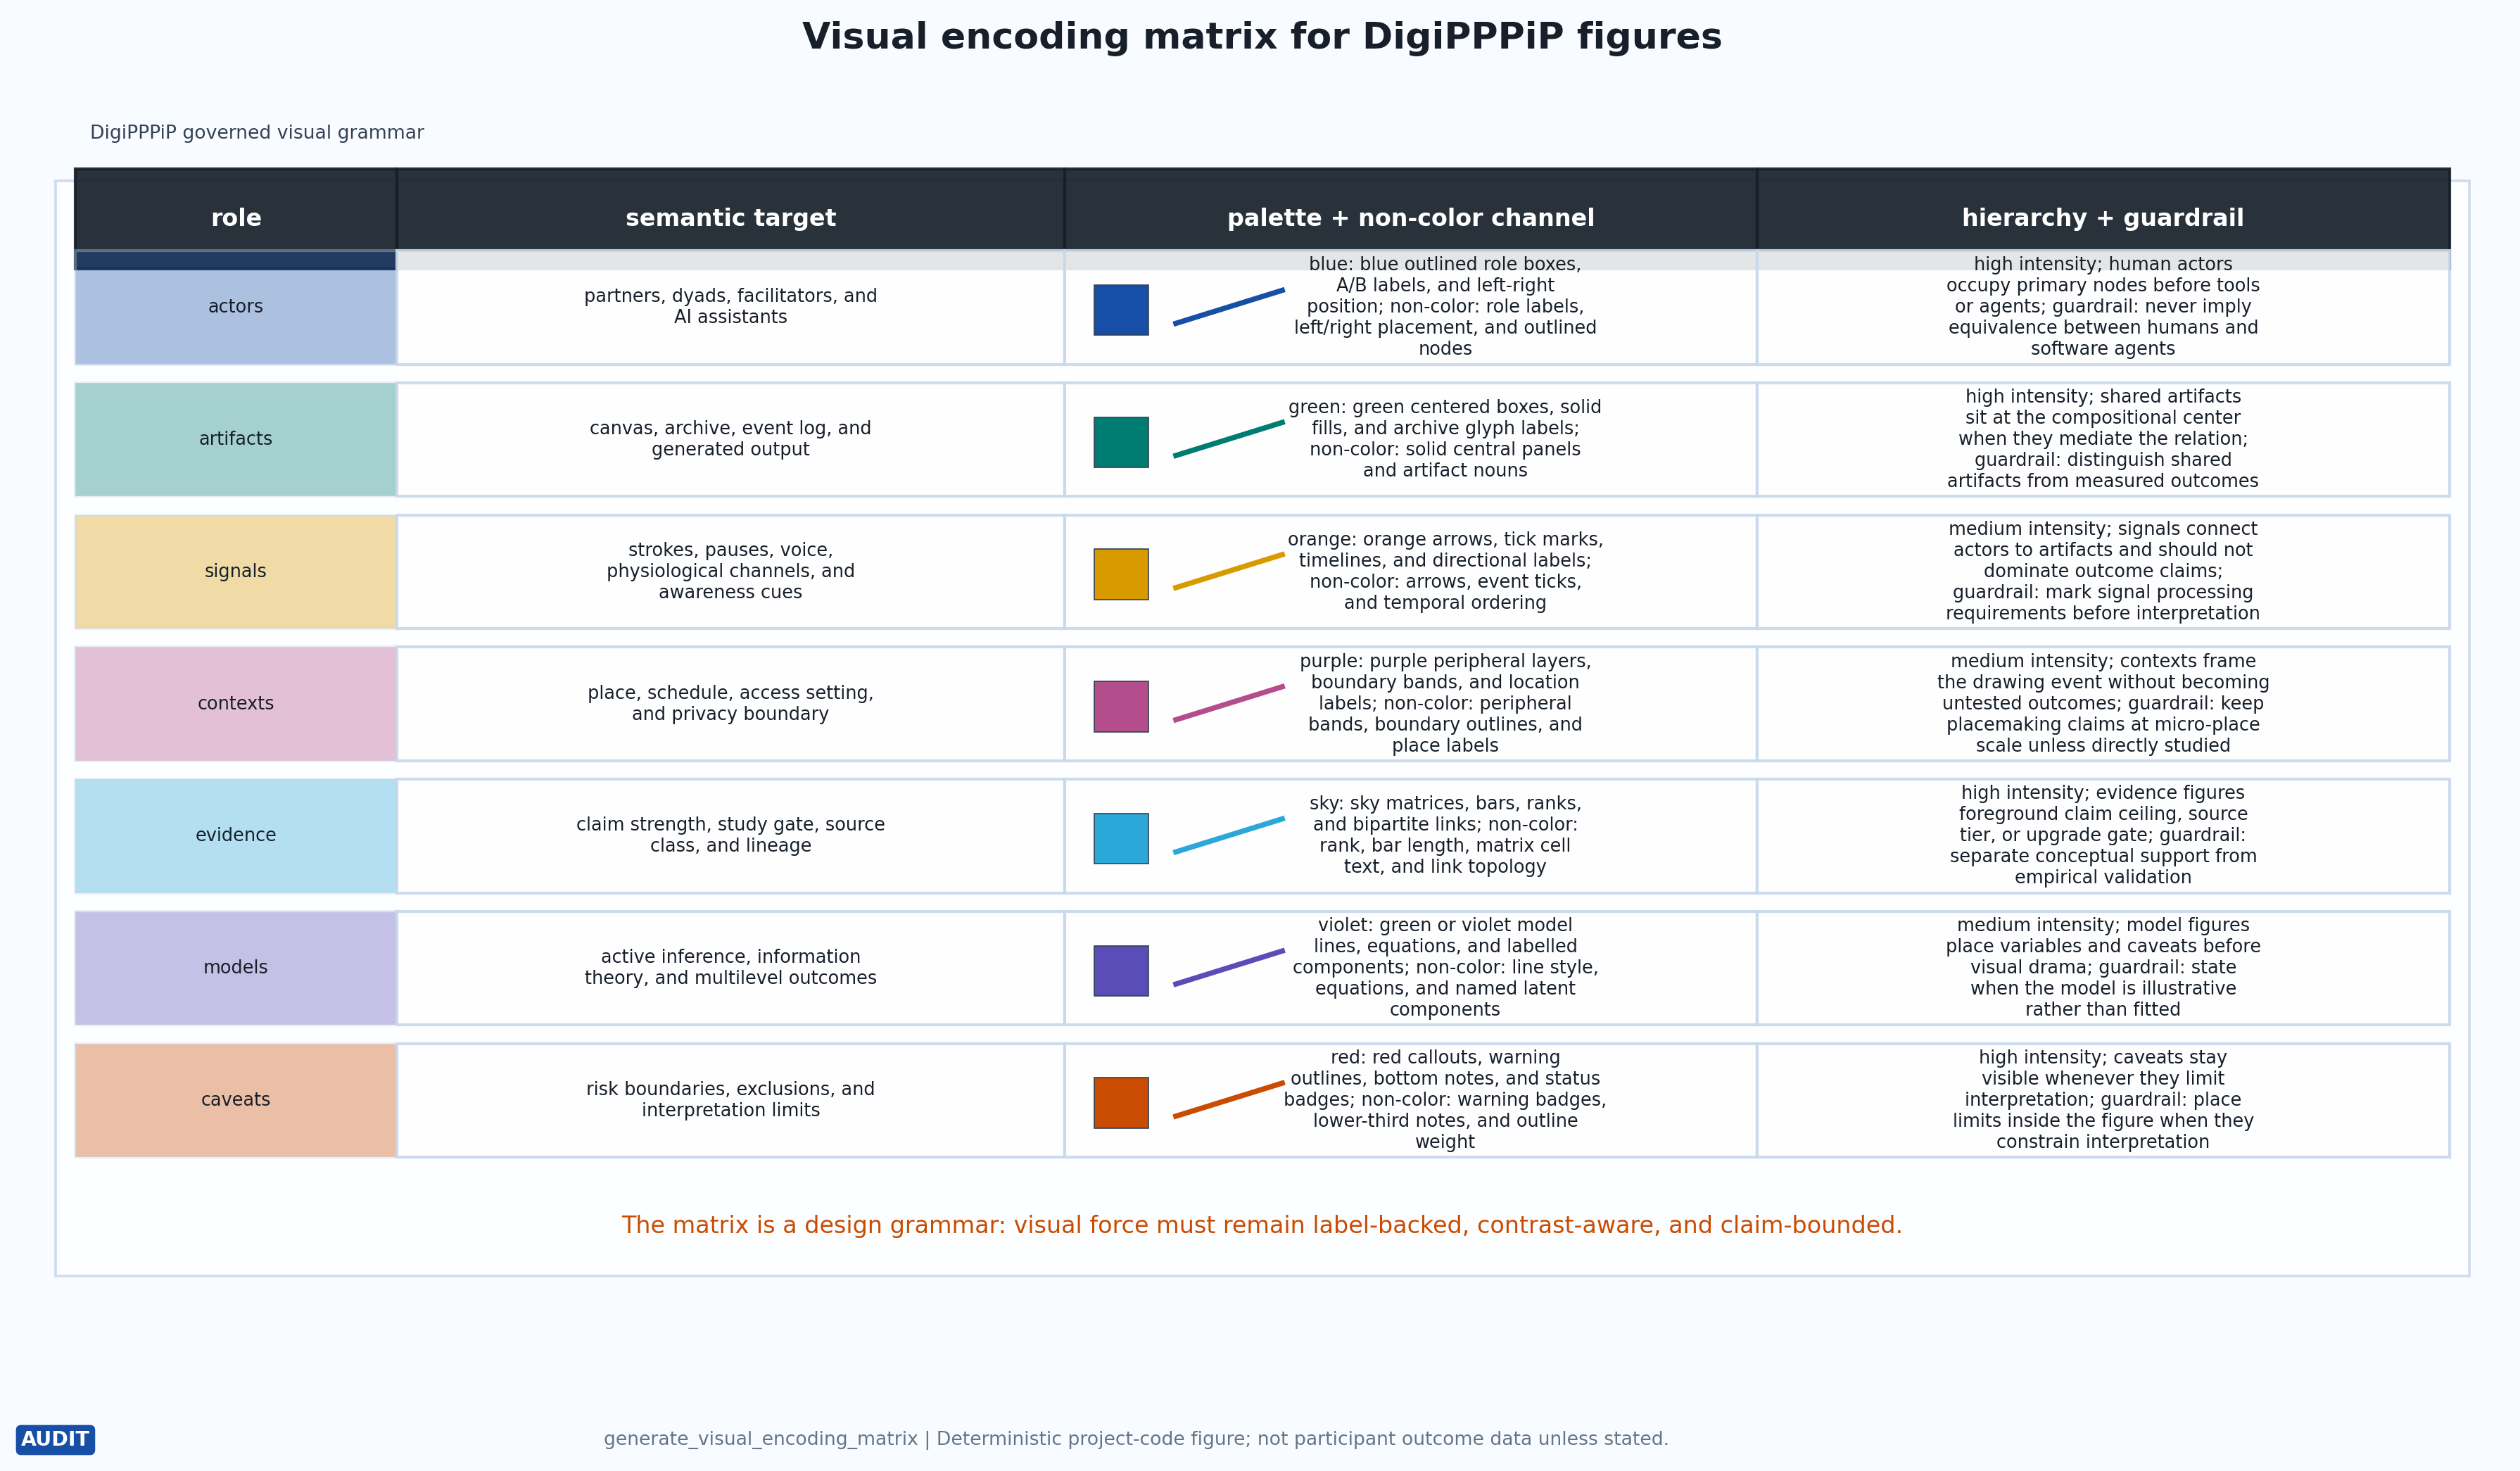
\includegraphics[width=0.95\linewidth,height=0.46\textheight,keepaspectratio,alt={Visual encoding matrix for generated DigiPPPiP figures. The matrix is generated by generate\_visual\_encoding\_matrix() from src/figure\_methods.py; read each row as a semantic role with its target, palette key, non-color channel, hierarchy rule, contrast cue, and interpretation guardrail. It supports the methods argument that repeated colors, labels, positions, marks, and text equivalents form a reusable grammar. The matrix is conceptual, and empirical data would add measured scales without removing the guardrails.}]{../figures/visual_encoding_matrix.png}
\caption{Visual encoding matrix for generated DigiPPPiP figures. The
matrix is generated by
\protect\breaktt{generate\_visual\_encoding\_matrix()} from
\protect\breaktt{src/figure\_methods.py}; read each row as a semantic
role with its target, palette key, non-color channel, hierarchy rule,
contrast cue, and interpretation guardrail. It supports the methods
argument that repeated colors, labels, positions, marks, and text
equivalents form a reusable grammar. The matrix is conceptual, and
empirical data would add measured scales without removing the
guardrails.}\label{fig:visual_encoding_matrix}
\end{figure}

\breakseq{[@fig:figure\_method\_audit]} then turns the caption and rendering
expectations into a checklist. The audit is not a guarantee that every
reader will understand every figure in the same way. It is a
reproducibility guard: a figure must name what it encodes, identify the
source or generator, state its method lineage and manuscript role,
explain how to read marks or axes, declare whether it is conceptual,
protocol, audit, analytic simulation, or empirical placeholder material,
preserve the caveat that limits interpretation, and identify what future
evidence would upgrade the claim. That requirement also improves
accessibility because natural-language descriptions can convey marks,
statistics, perceptual relations, and domain meaning for readers who
cannot rely on the image alone \breakseq{[@lundgard2022accessible]}. Current
accessible-visualization work extends the requirement from alt text
toward navigable structure, customizable token order, and
reader-controlled verbosity \breakseq{[@elavsky2024datanavigator;
@jones2024customization]}. The code now writes long-description
sidecars for every generated figure and emits
\breaktt{output/figures/figure\_artifact\_audit.json}, an artifact-level
audit that checks registry uniqueness, orphan PNGs, dimensions, nonblank
pixels, manuscript references, caption/prose parity, claim-status
validity, long-description presence, readability metadata,
long-description reading guidance, and section alignment after the
figure set is rendered.

\begin{figure}
\centering
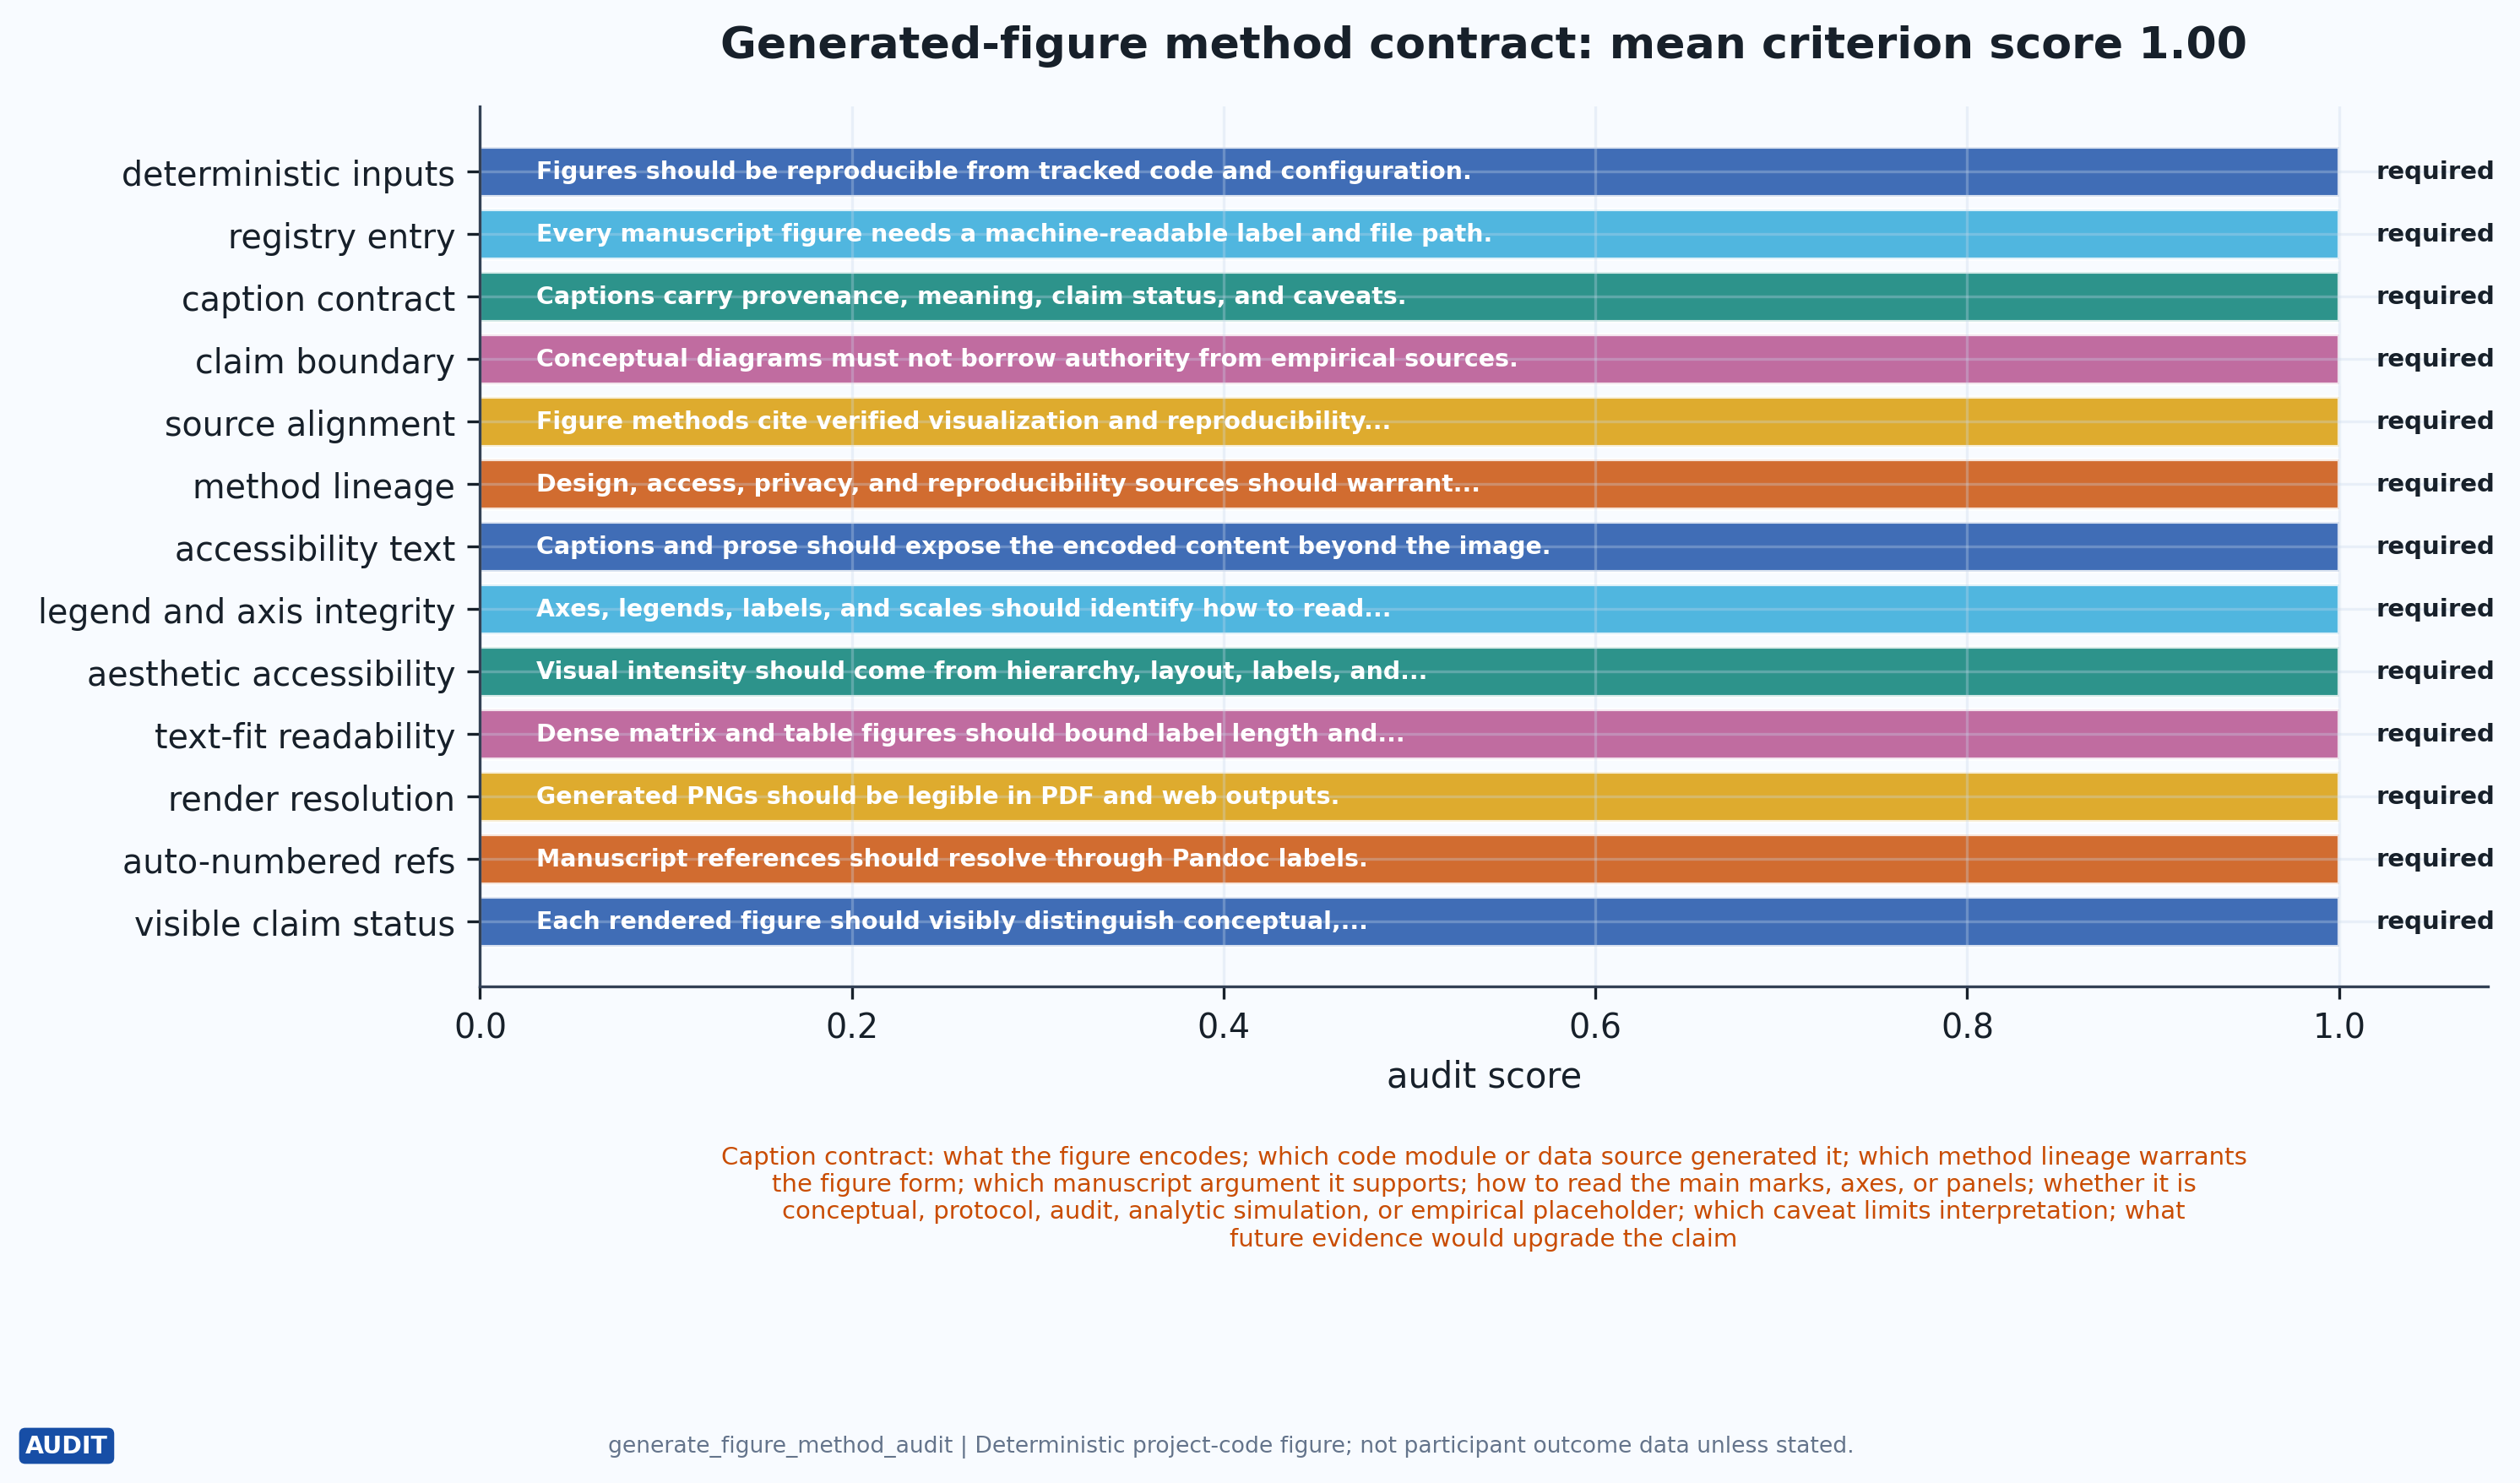
\includegraphics[width=0.9\linewidth,height=0.46\textheight,keepaspectratio,alt={Figure-method audit for DigiPPPiP generated figures. Bars are generated by generate\_figure\_method\_audit() from src/figure\_methods.py; read each row as a required gate covering deterministic inputs, registry metadata, captions, claim boundaries, source alignment, accessibility text, legend/axis integrity, render resolution, auto-numbered references, and visible claim status. It supports workflow verification, not participant inference. Failed gates would require code or caption repair.}]{../figures/figure_method_audit.png}
\caption{Figure-method audit for DigiPPPiP generated figures. Bars are
generated by \protect\breaktt{generate\_figure\_method\_audit()} from
\protect\breaktt{src/figure\_methods.py}; read each row as a required
gate covering deterministic inputs, registry metadata, captions, claim
boundaries, source alignment, accessibility text, legend/axis integrity,
render resolution, auto-numbered references, and visible claim status.
It supports workflow verification, not participant inference. Failed
gates would require code or caption
repair.}\label{fig:figure_method_audit}
\end{figure}
\end{frame}

\begin{frame}[fragile,allowframebreaks]{Study Package, Access, Place,
and Outcomes}
\protect\phantomsection\label{study-package-access-place-and-outcomes}
The minimum reproducibility package for a DigiPPPiP study should include
the protocol version, temporal-spatial condition, interface
capabilities, event schema, exclusion windows, consent and persistence
settings, accessibility accommodations, outcome measures, and analysis
code. Without that package, readers cannot tell whether an observed
result belongs to the dyad, the task, the technology, the access
arrangement, or the analysis pipeline. This is a first-principles
requirement: if the causal candidates cannot be separated, the
interpretation cannot be audited.

The protocol appendix should also separate three participant-facing
surfaces that are easy to collapse. The access surface records supported
input channels, feedback channels, partner-mediated assistance,
cognitive-load settings, communication preferences, and accommodation
changes during the session. The place surface records only the situated
cues that participants consent to share, such as room type, local
prompt, mobility context, or remembered place, and it should not require
precise geolocation for a place-responsive claim. The health surface
states that DigiPPPiP is non-clinical unless a reviewed intervention
protocol says otherwise, names stop and referral procedures, and
separates personal keepsakes from research logs before any export or
replay.

Reporting guidance supplies the study-readiness bridge. The Template for
Intervention Description and Replication (TIDieR) requires enough
intervention detail for replication, and the Consolidated Standards of
Reporting Trials for eHealth (CONSORT-EHEALTH) names web and mobile
health reporting elements that are easy to miss when an online
intervention feels self-explanatory \breakseq{[@hoffmann2014tidier;
@eysenbach2011consortehealth]}. For DigiPPPiP that means the protocol
must define session dose, materials, platform settings, tailoring,
fidelity, archive-control states, and changes made during the study. The
Preferred Reporting Items for Systematic Reviews and Meta-Analyses
(PRISMA) is not activated here because the evidence graph is a bounded
narrative synthesis rather than a systematic review claim; it should be
added only if the review question, search strategy, screening,
extraction, and flow diagram become systematic.

Accessibility is handled as a protocol requirement. The current audit
has 5 criteria and an illustrative implementation score of 1. The radar
in \breakseq{[@fig:accessibility\_audit\_radar]} is not a compliance
certificate; it is a reproducible way to document which input, feedback,
privacy, cognitive-load, and partner-mediation capabilities a study or
tool actually supports.

\begin{figure}
\centering
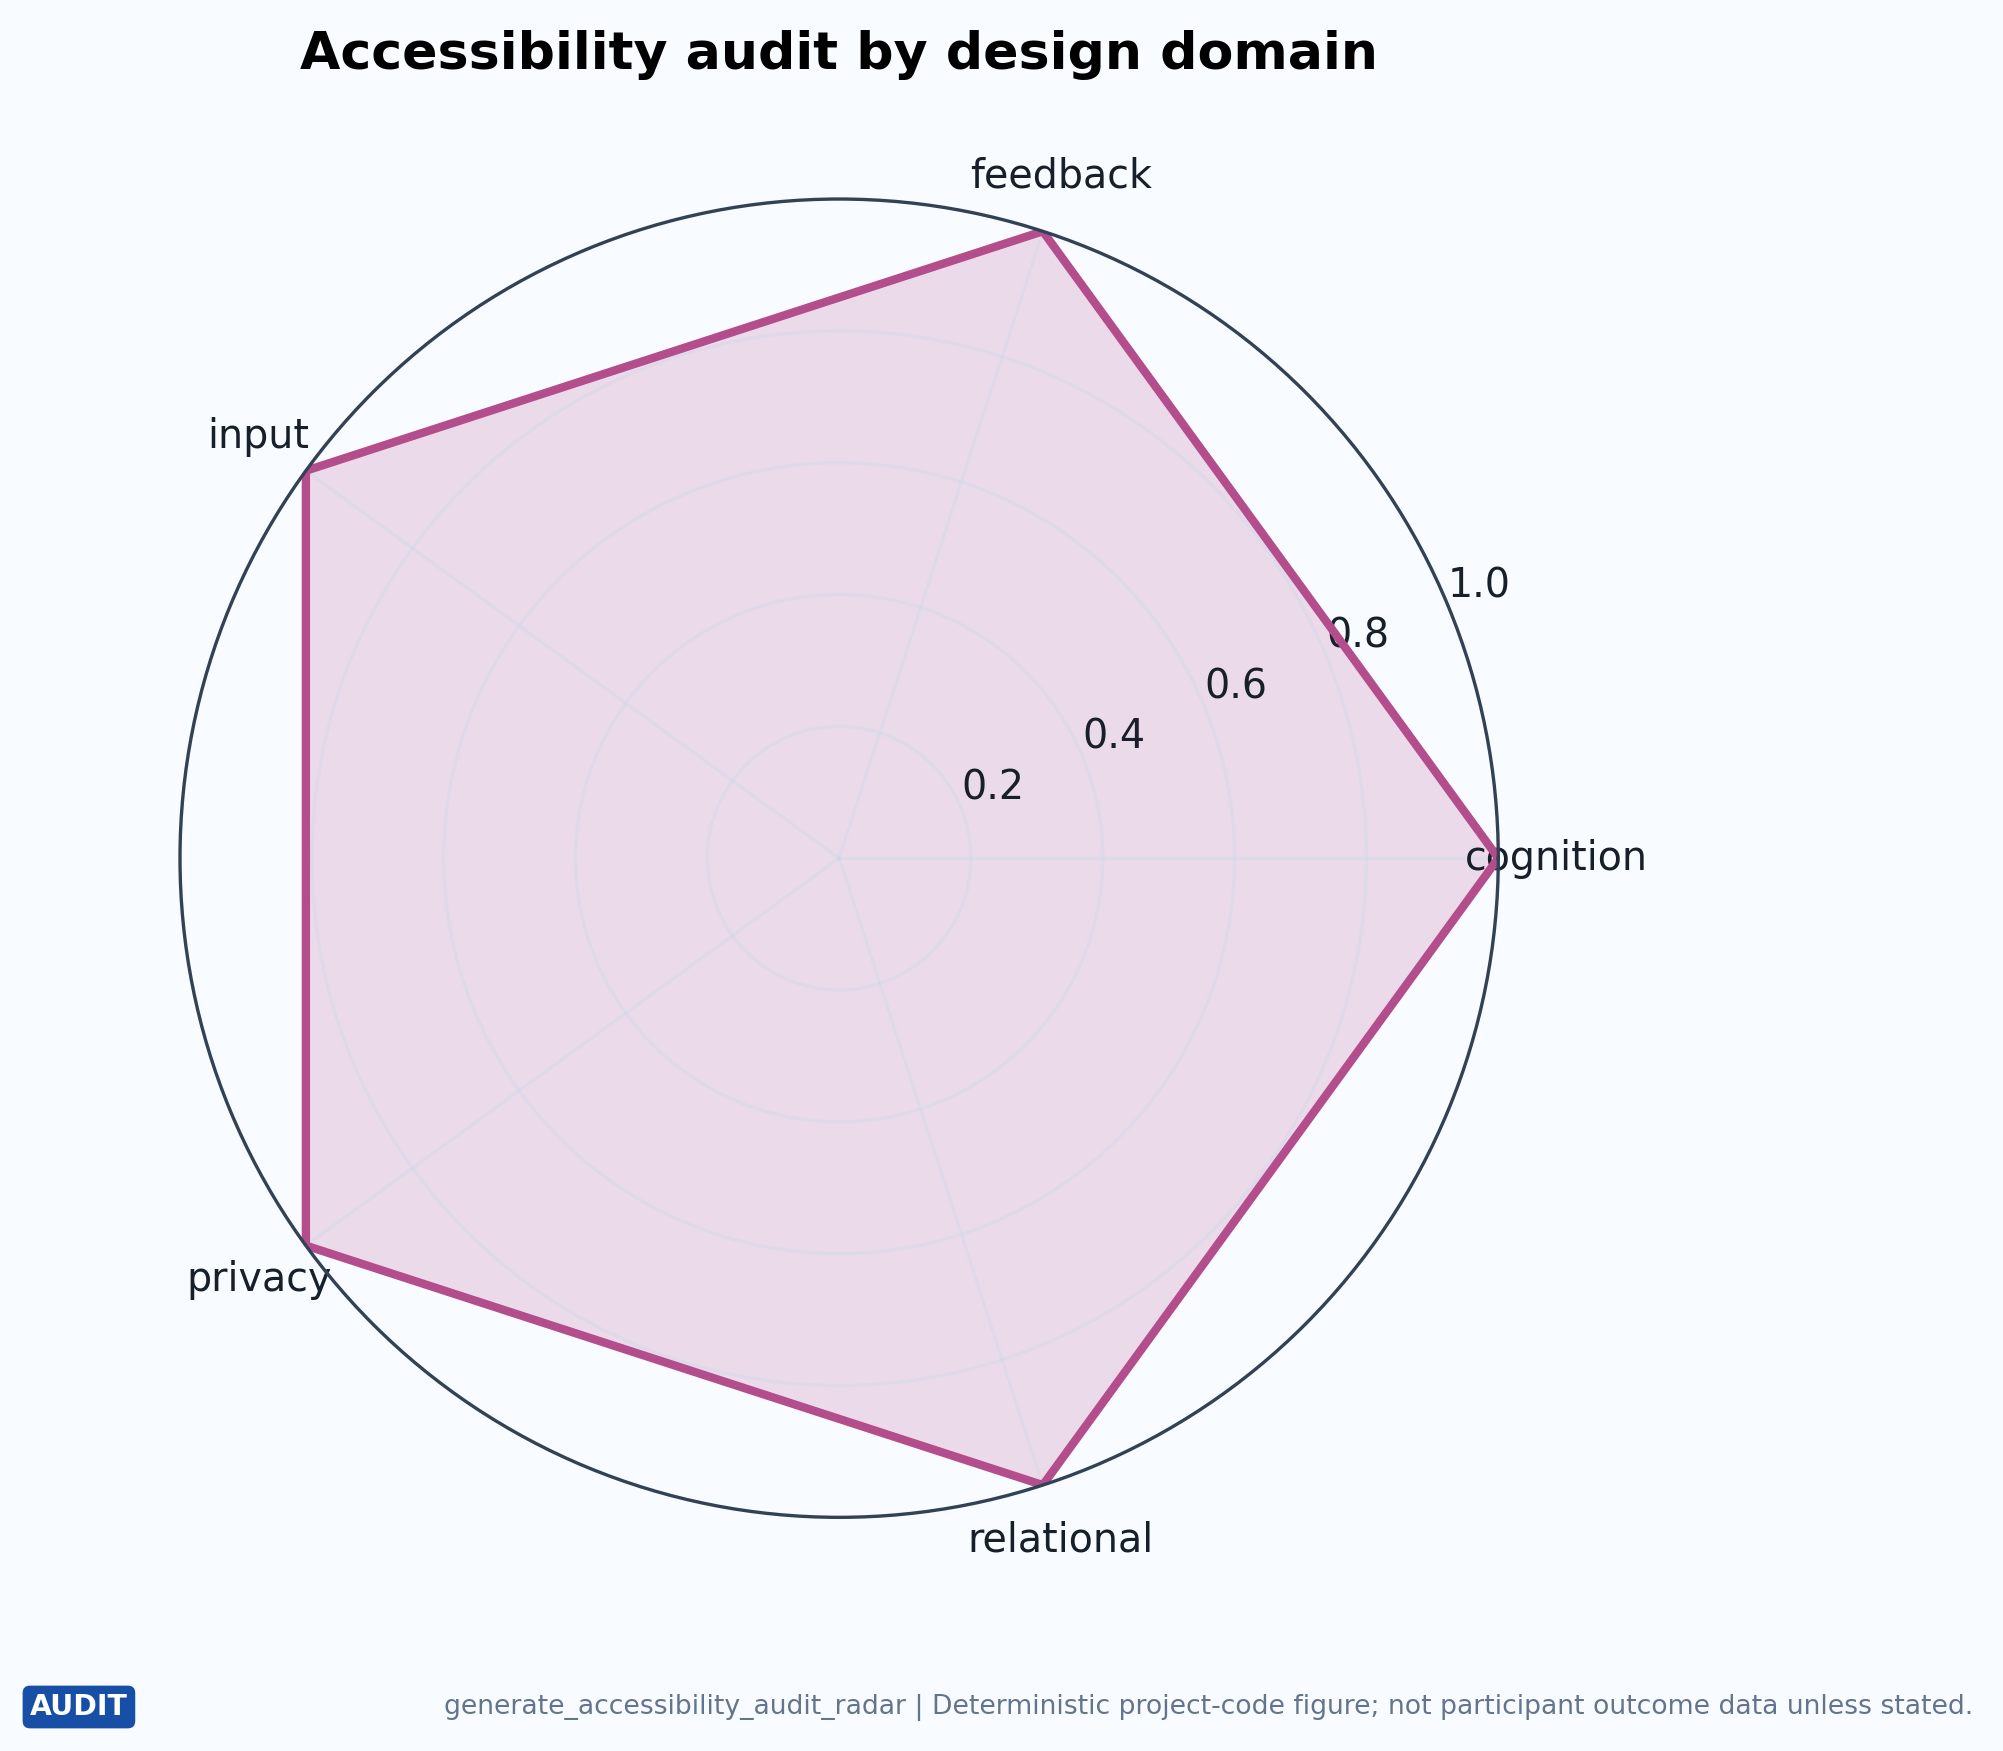
\includegraphics[width=0.75\linewidth,height=0.46\textheight,keepaspectratio,alt={Accessibility audit radar generated from explicit implementation capabilities. The figure is generated by generate\_accessibility\_audit\_radar() from src/accessibility.py; read each spoke as a capability domain and radial distance as documented support in the illustrative configuration. It supports reproducible access auditing, not compliance certification. Empirical accessibility claims would require participatory validation with disabled users and accommodation logs.}]{../figures/accessibility_audit_radar.png}
\caption{Accessibility audit radar generated from explicit
implementation capabilities. The figure is generated by
\protect\breaktt{generate\_accessibility\_audit\_radar()} from
\protect\breaktt{src/accessibility.py}; read each spoke as a capability
domain and radial distance as documented support in the illustrative
configuration. It supports reproducible access auditing, not compliance
certification. Empirical accessibility claims would require
participatory validation with disabled users and accommodation
logs.}\label{fig:accessibility_audit_radar}
\end{figure}

Outcomes are organized as a multilevel design rather than a single
success metric. The project defines 6 measures across 6 domains, with a
default design-strength score of 4 for a randomized longitudinal study.
\breakseq{[@fig:multilevel\_outcome\_model]} shows how temporal mode, spatial
configuration, phase, and access condition can be modeled with dyad and
participant random effects. This structure separates implementation
outcomes, such as latency and logging completeness, from relational
outcomes, such as perceived connection and shared meaning.

\begin{figure}
\centering
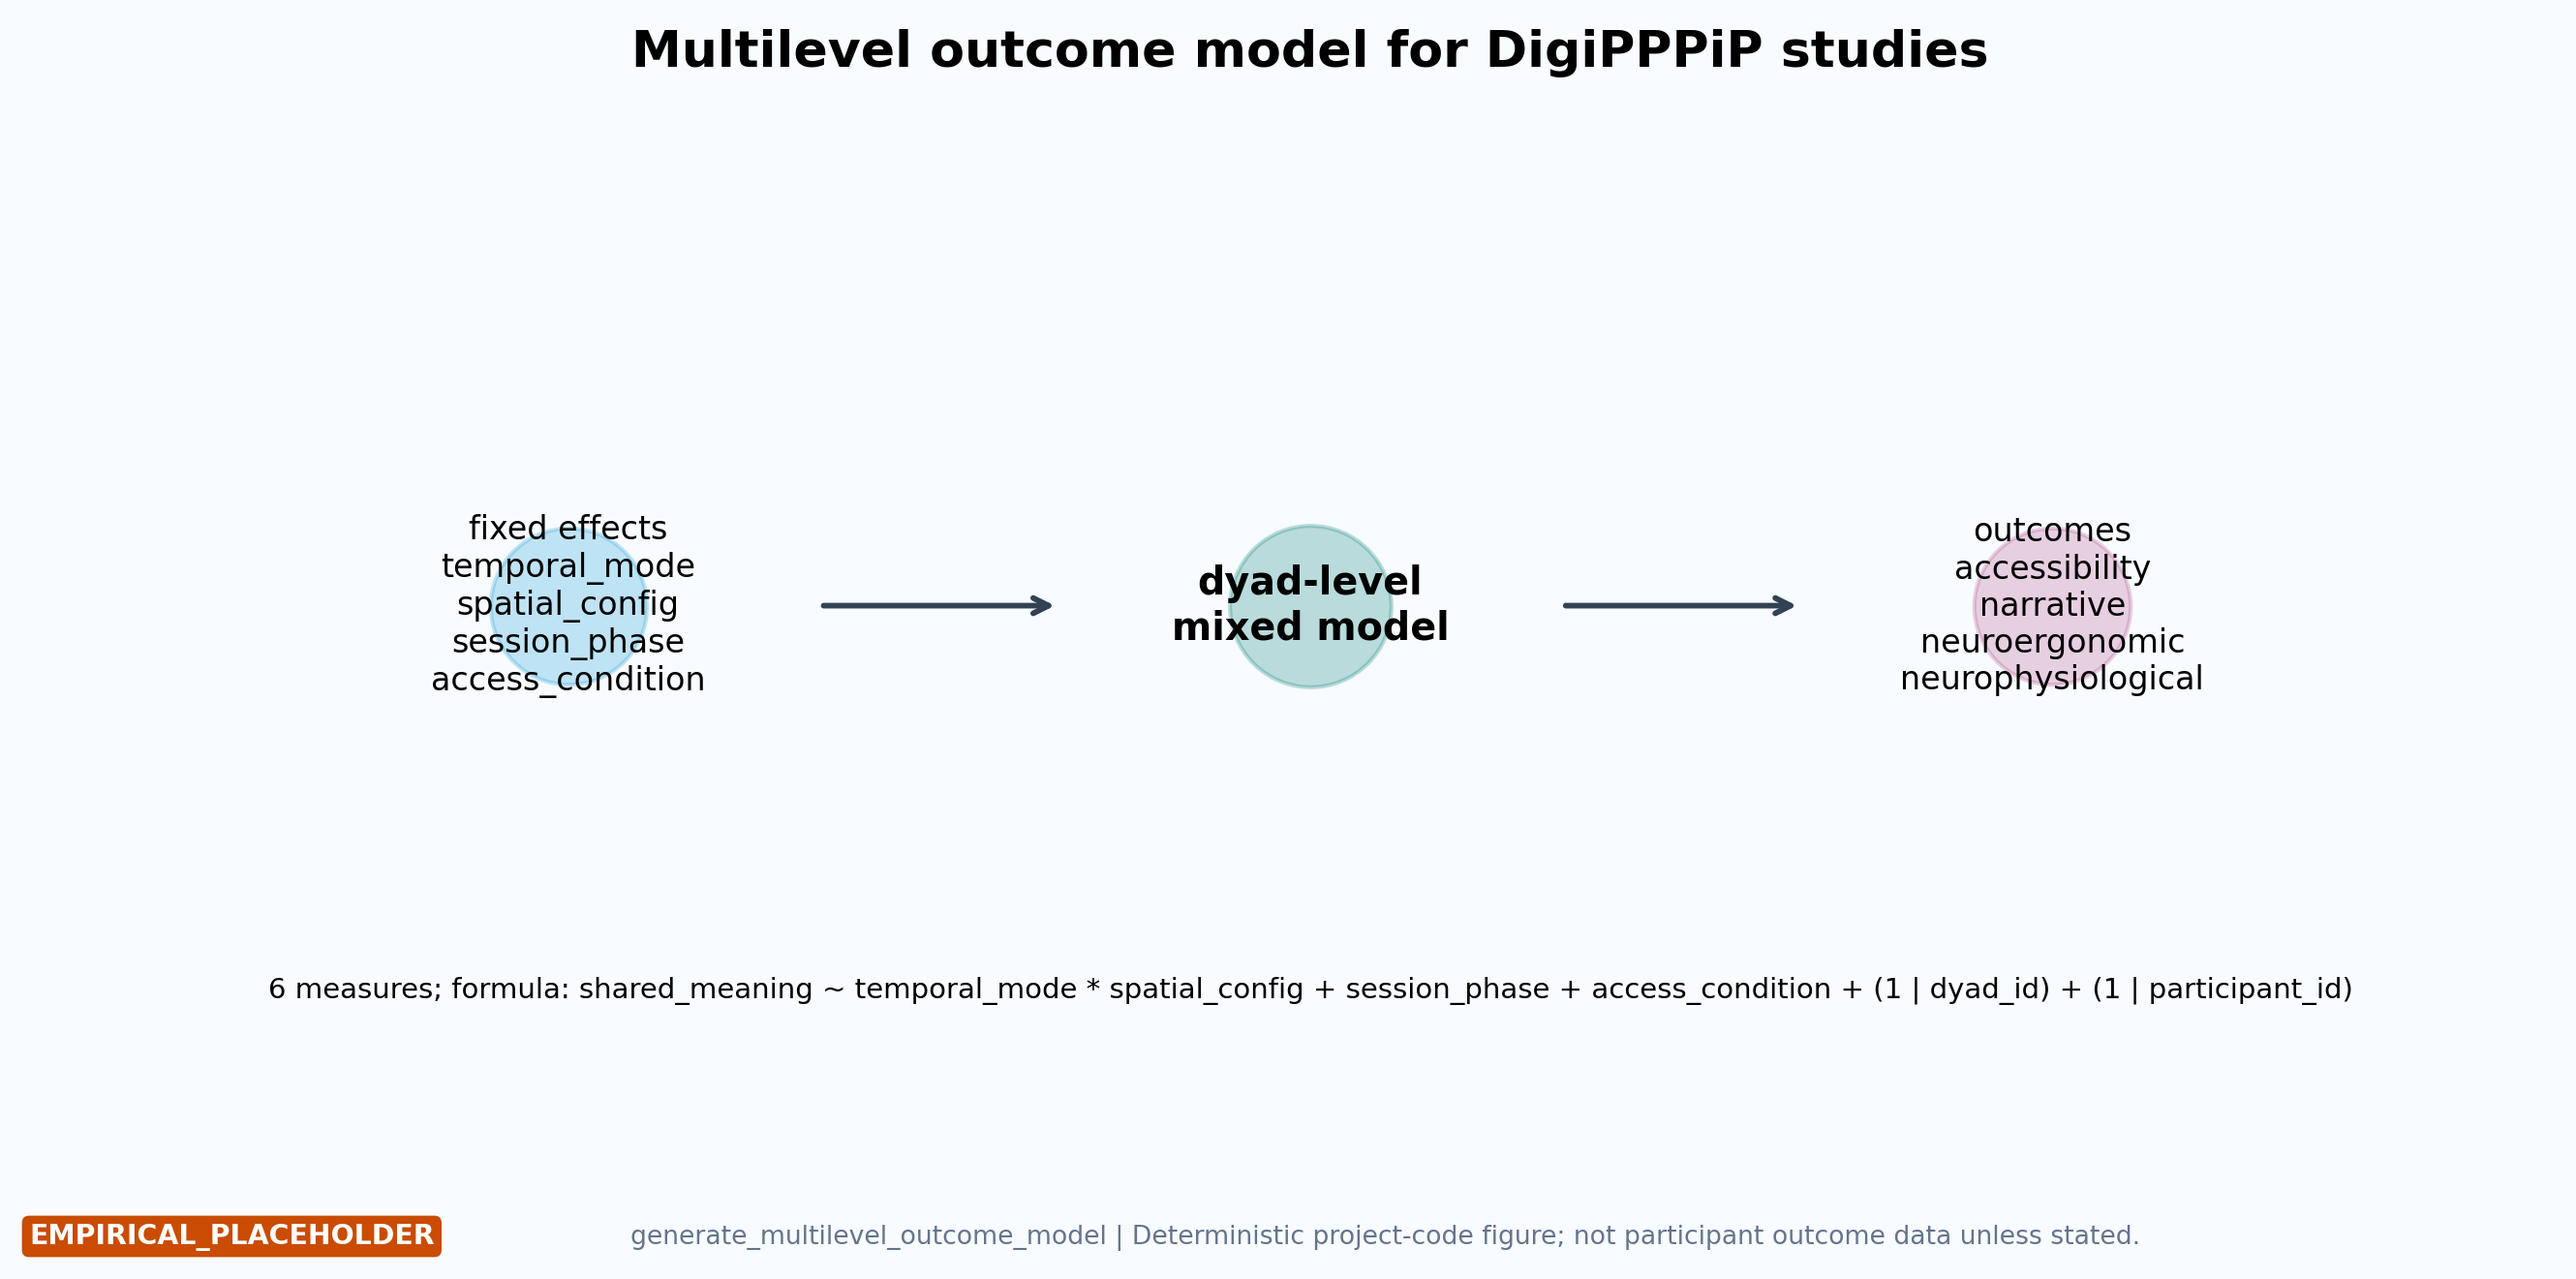
\includegraphics[width=0.9\linewidth,height=0.46\textheight,keepaspectratio,alt={Multilevel outcome model for DigiPPPiP studies. The figure is generated by generate\_multilevel\_outcome\_model() from src/outcomes.py; read left components as fixed effects, the center as the dyad-level mixed model, and the right component as outcome domains. It supports planned-analysis specification rather than reporting results. Validation would require real dyadic observations, random effects diagnostics, and matched shared-activity controls.}]{../figures/multilevel_outcome_model.png}
\caption{Multilevel outcome model for DigiPPPiP studies. The figure is
generated by \protect\breaktt{generate\_multilevel\_outcome\_model()}
from \protect\texttt{src/outcomes.py}; read left components as fixed
effects, the center as the dyad-level mixed model, and the right
component as outcome domains. It supports planned-analysis specification
rather than reporting results. Validation would require real dyadic
observations, random effects diagnostics, and matched shared-activity
controls.}\label{fig:multilevel_outcome_model}
\end{figure}
\end{frame}

\begin{frame}[fragile,allowframebreaks]{Falsification and Claim
Boundaries}
\protect\phantomsection\label{falsification-and-claim-boundaries}
Falsification should be designed in. The framework would be weakened if
matched controls produce the same relational outcomes, if accessibility
accommodations reduce rather than expand agency, if synchrony measures
vanish after artifact correction, if AI suggestions displace rather than
support human agency, or if participants describe persistent archives as
surveillance rather than shared memory. Those outcomes would not
invalidate shared drawing as a practice; they would delimit which
mechanisms, contexts, or claims the framework can support.

\breakseq{[@fig:validation\_ladder]} expresses this as 5 staged gates.
Feasibility and relational meaning come before access claims, matched
outcome comparisons, and optional physiology. This ordering is
adversarial by design: neural or computational sophistication cannot
rescue a practice that is not understood, consentful, accessible to the
stated population, or meaningfully different from simpler shared
activities.

\begin{figure}
\centering
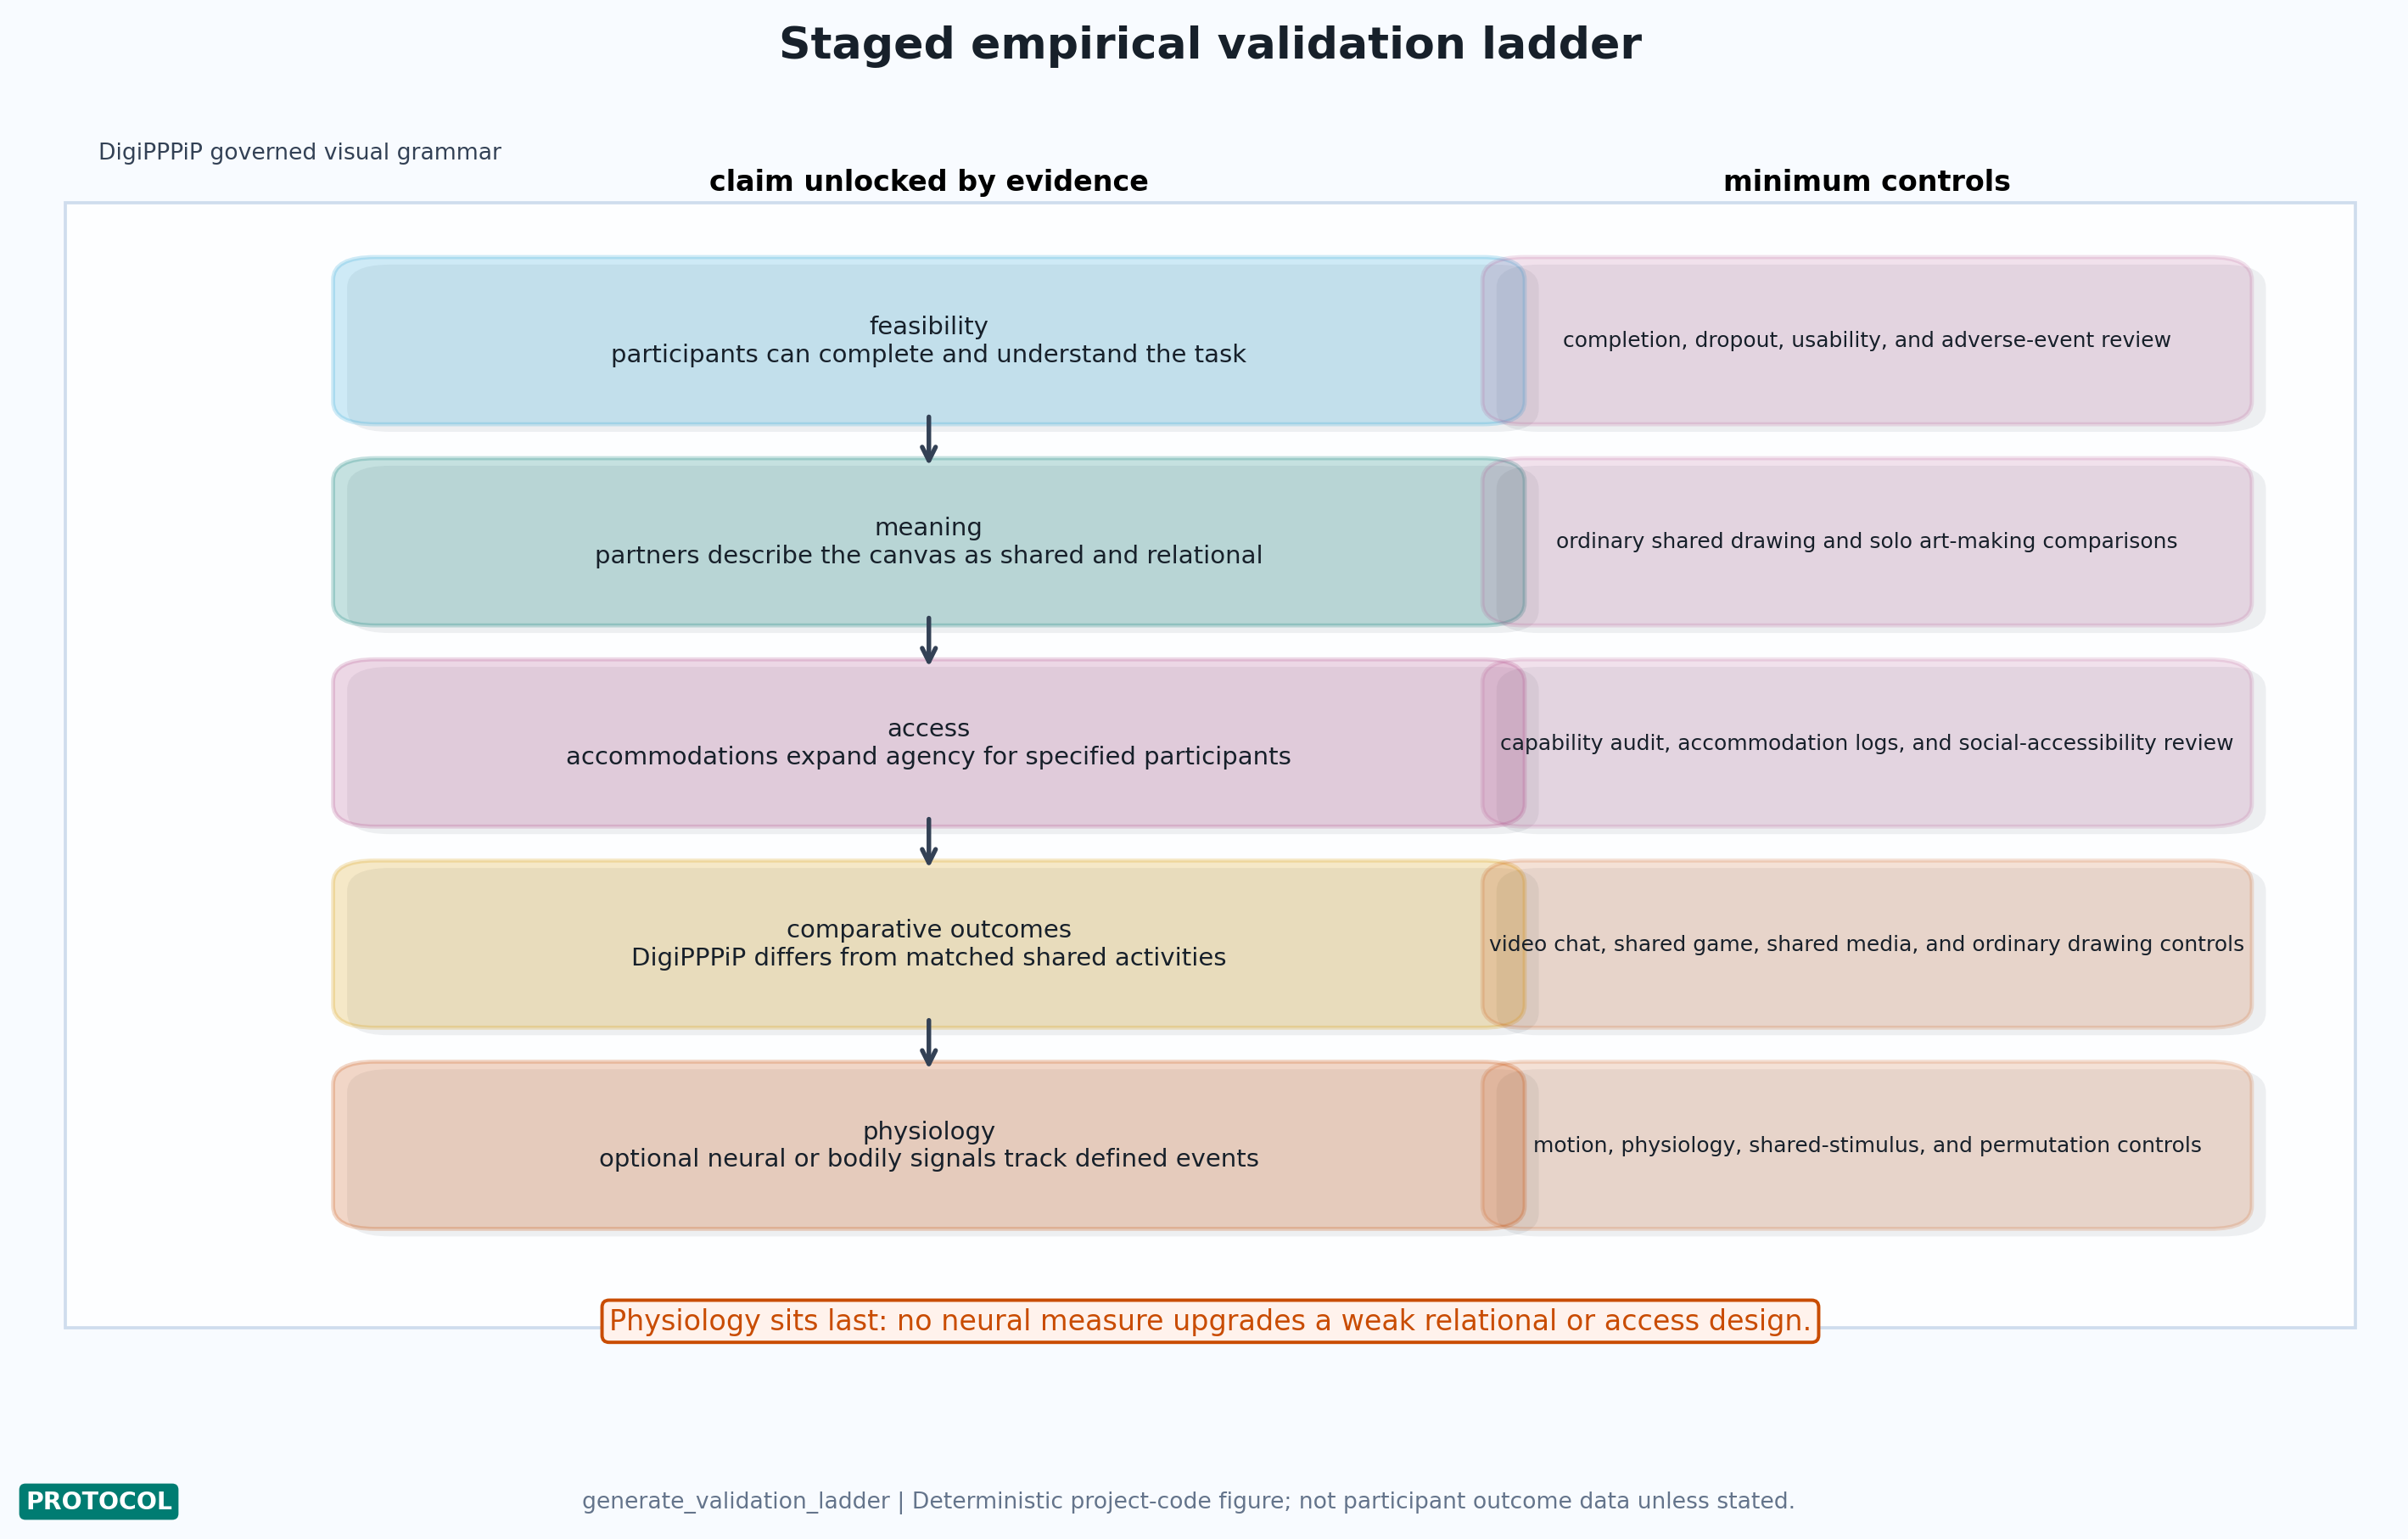
\includegraphics[width=0.9\linewidth,height=0.46\textheight,keepaspectratio,alt={Staged empirical validation ladder for DigiPPPiP. The figure is generated by generate\_validation\_ladder() from src/source\_quality.py; read the left column as claims unlocked by each stage and the right column as minimum controls before escalation. It supports the protocol's adversarial ordering from feasibility and meaning through access, matched outcomes, and optional physiology. The ladder is conceptual, and stronger claims require completed studies at the relevant stage.}]{../figures/validation_ladder.png}
\caption{Staged empirical validation ladder for DigiPPPiP. The figure is
generated by \protect\breaktt{generate\_validation\_ladder()} from
\protect\breaktt{src/source\_quality.py}; read the left column as claims
unlocked by each stage and the right column as minimum controls before
escalation. It supports the protocol's adversarial ordering from
feasibility and meaning through access, matched outcomes, and optional
physiology. The ladder is conceptual, and stronger claims require
completed studies at the relevant stage.}\label{fig:validation_ladder}
\end{figure}

This protocol prevents the main evidentiary errors. Active inference is
used as a modeling language, not proof of mechanism. Hyperscanning
synchrony is treated as a correlate until causal designs justify more
\breakseq{[@cui2012nirs; @czeszumski2020hyperscanning;
@hamilton2021hyperscanning; @zimmermann2024methodological]}.
Art-therapy and digital-health literatures motivate possible
applications and cautions, but DigiPPPiP is not described as treatment
without controlled clinical evidence \breakseq{[@zubala2021digitalarttherapy]}.
Accessibility and placemaking claims stay bounded to the capabilities
and populations actually tested.
\end{frame}

\end{document}
